\documentclass[conference]{IEEEtran}
\IEEEoverridecommandlockouts
% The preceding line is only needed to identify funding in the first footnote. If that is unneeded, please comment it out.
\usepackage{cite}
\usepackage{amsmath,amssymb,amsfonts}
\usepackage{algorithmic}
\usepackage{graphicx}
\usepackage{textcomp}
\usepackage{xcolor}
\usepackage{caption}
\usepackage{subcaption}
\usepackage[left=0.680in, right=0.620in, bottom = 1in, top=0.7in]{geometry}
\usepackage{url,amssymb,threeparttable,multirow,booktabs, tabularx}
\def\BibTeX{{\rm B\kern-.05em{\sc i\kern-.025em b}\kern-.08em
    T\kern-.1667em\lower.7ex\hbox{E}\kern-.125emX}}
\usepackage{algpseudocode} 
\usepackage{algorithm} 


\captionsetup[table]{font=footnotesize}
\captionsetup[figure]{font=footnotesize}


\begin{document}

\title{Optimum Multiuser Modulation and Coding for Energy-Efficient Extended Reality (XR) Support\\
}

\author{
\IEEEauthorblockN{Sagnik Bhattacharya\textsuperscript{1}, Kamyar Rajabalifardi\textsuperscript{1}, Rohan Pote\textsuperscript{2}, Hyukjoon Kwon\textsuperscript{2}, Dongwoon Bai\textsuperscript{2}, John M. Cioffi\textsuperscript{1}}

\IEEEauthorblockA{\textsuperscript{1}Dept. of Electrical Engineering, Stanford University, Stanford, CA, USA} 

\IEEEauthorblockA{\textsuperscript{2}Samsung Semiconductors, San Diego, CA, USA} 

\IEEEauthorblockA{
% \textit{Dept. of Electrical Engineering, Stanford University, CA, U.S.A} \\
Emails: \{sagnikb, kfardi, cioffi\}@stanford.edu, \{rohan.pote, hyukjoon.k, dongwoon.bai\}@samsung.com}
}

\maketitle
\vspace{-40pt}

\begin{abstract}
In the ever-evolving landscape of Extended Reality (XR)-based distributed rendering, the scenario where the number of user antennas exceeds the number of access point (AP) antennas presents a low-rank channel problem. This often arising situation demands high data rates (upto 500 Mbps) and low power consumption. Current Wi-Fi solutions using OFDM-based power allocation fall short in addressing these requirements efficiently. This paper introduces a novel non-linear Generalized Decision Feedback Equalizer (GDFE) based algorithm to optimize the power allocation to elevate data rates and minimize energy usage,  especially in low rank scenarios. Incorporating time-sharing techniques, the proposed algorithm offers substantial improvements over existing standards. Extensive experimental validations highlight its ability to significantly outperform contemporary Wi-Fi methods, marking a step forward in enabling advanced XR applications.
\end{abstract}

\begin{IEEEkeywords}
extended reality (XR), augmented reality (AR), generalized decision feedback equalizer (GDFE), multiple access channel (MAC), time sharing
\end{IEEEkeywords}

% \section{Introduction}

% Wireless communication is critically important in augmented reality (AR) and virtual reality (VR) devices, primarily due to the resource-intensive nature of data processing in these edge devices. AR and VR technologies demand high computational power to render complex, immersive environments in real-time, which can be exceedingly demanding for the processors within the devices. Wireless communication can offload these computationally intensive tasks to powerful servers. This server-side processing approach allows for handling complex calculations and rendering tasks, which are then efficiently transmitted back to the edge device. This not only enhances the performance and capabilities of AR/VR devices but also significantly reduces the hardware requirements and power consumption at the user's end. In this regard, we will introduce the minPMAC algorithm to allocate the optimal data rate to each user based on the energy constraint and their distance to the access point (AP).

% write on XR systems advancement
XR (Extended Reality), encompassing AR (Augmented Reality), VR (Virtual Reality), and mixed reality, is revolutionizing how we interact with digital content, merging virtual and real worlds for enhanced experiences in education, healthcare, and entertainment \cite{xr1, xr2, xr3, xr4}. In a broader perspective, XR harbors the capability to supplant traditional computing devices, positioning itself as a ubiquitous computing platform. The full potential of XR technologies hinges on the development and deployment of low latency, low power, high bandwidth wireless communication systems. Such systems are crucial for delivering seamless, real-time experiences, minimizing delays that can disrupt immersion and user comfort. High bandwidth ensures rich, detailed virtual environments, while low power consumption is essential for the portability and longevity of wearable XR devices, making these technologies more accessible and effective in everyday applications.



% write on distributed rendering problem
In our research, we address the distributed rendering challenge in Extended Reality (XR) systems \cite{rendering1}, with a focus on Virtual Reality (VR) environments. We examine a scenario involving \( N \) users, each equipped with resource-limited VR headsets, engaging in a collaborative VR gaming experience. These users, distributed within a virtual room, observe distinct segments of the environment, resulting in individual partial views. These fragmented visual inputs are then transmitted to a central processing server via uplink connections using Wi-Fi 7 technology. The central server, endowed with substantial computational capabilities, employs advanced image processing algorithms to amalgamate these disparate visual fragments into a cohesive three-dimensional spatial representation of the room. Upon successful synthesis of a complete 3D map, the server redistributes this integrated visual content back to the users through a high-speed downlink Wi-Fi channel. This process ensures that participants in the VR environment receive a seamless, uninterrupted 360-degree panoramic view, thereby enhancing the immersive quality of the virtual experience in real-time.

The uplink distributed rendering scenario is a multiple-input-multiple-output (MIMO) multiple-access channel (MAC). The multiple-access channel is a fundamental model in communication, characterizing a situation where multiple transmitters are sending information to a single receiver. The uplink MIMO system with additive white gaussian noise (AWGN) can be expressed as:
\begin{equation}
    \boldsymbol{y} = H\cdot \boldsymbol{x} + \boldsymbol{n}
\end{equation}
Where $\boldsymbol{n}$ is the Gaussian noise, and $\boldsymbol{x}$, $\boldsymbol{y}$ are the transmitted and received signals, respectively. 


% write on 500 Mbps problem
Two primary challenges emerge as significant roadblocks for distributed XR rendering: the constraints of uplink communication bandwidth \cite{impediment1} and the considerable power consumption at edge devices, which are inherently resource-constrained \cite{impediment2}. XR heavily relies on Head-Mounted Displays (HMDs), which necessitate stringent adherence to power and weight limitations. The imperative to optimize the Quality-of-Experience (QoE) mandates that HMDs be lightweight and compact. Consequently, this necessitates the offloading of substantial computing and storage tasks to external processing units, such as computers or cloud-based servers. The transmission of complex three-dimensional imagery, a cornerstone of these VR applications, necessitates data rates reaching upwards of 500 Mbps per user antenna. However, the capabilities of existing wireless communication protocols, even those conforming to the latest Wi-Fi standards (802.11b/g/n/ac) \cite{wifi1, wifi2}, are insufficient for such high data rate demands, especially when the number of antennas at the users exceeds the number of antennas at the access point (AP), and/or the channel is low rank. This issue makes the task of transmitting uplink 3D image data impractical. Additionally, the current achievable data rates through Wi-Fi, while substantial, lead to prohibitive power consumption levels. This scenario is particularly challenging for devices like Augmented Reality (AR) glasses, where limited power resources are a critical constraint. These limitations significantly impede the development and practical realization of XR systems dependent on intense and real-time data transmission for distributed rendering in VR environments.

% write on prior work to address problem


% write on proposed solution (cite ellipsoid and GDFE papers)
In this paper, we address these challenges by optimizing the data rates and the power consumption using a non-linear generalized decision feedback equalizer (GDFE) \cite{gdfe, yunGlobecom}. {\color{red} write little more on algorithm details} We achieve the maximum possible data rates for each of the \( N \) users in a VR setting, considering factors such as the channel impulse responses between the users and the AP, the number of antennas, the distance from the AP, and the transmit signal-to-noise ratio at each user's device. In a converse approach, given the prerequisite minimum data rates necessary for each user, our objective is to minimize the power consumption at each of these edge devices. We show that the proposed GDFE-based solutions achieve much higher data rates with much lower power consumption, compared to current Wi-Fi standards, using the time-sharing (vertex sharing) technique. Through this dual optimization strategy, we endeavor to overcome the prevailing bottlenecks in uplink communication capacity, thereby paving the way for the development and deployment of high-fidelity XR systems.

% write on metrics we outperform on
We undertake a series of extensive experiments to rigorously evaluate the performance of our proposed distributed rendering system for Extended Reality (XR) applications. These experiments are meticulously designed to encompass a broad range of parameters, including channel impulse responses, the number of users involved, the quantity of antennas per user, requisite minimum data rates, signal-to-noise ratio (SNR), and the spatial distances from the access point (AP). We compare the results of the proposed GDFE-based algorithm to the traditional Orthogonal Frequency Division Multiplexing (OFDM)-based Wi-Fi standards.

Our results demonstrate a significant enhancement in achievable data rates with the implementation of the GDFE-based algorithm, reaching upwards of 500 Mbps per user antenna. This figure notably surpasses the data rates feasible through traditional Wi-Fi methodologies. Furthermore, our analysis reveals a substantial improvement in power efficiency. Specifically, for a given minimum required data rate — a threshold that traditional Wi-Fi can accomplish — our proposed algorithm demonstrates the capability to achieve this benchmark with an order of magnitude lower power consumption on the user devices. This finding is particularly impactful, considering the constraints of power resources in edge devices such as Augmented Reality (AR) glasses, commonly employed in XR systems. These experimental outcomes underscore the superiority of our proposed algorithm, not only in terms of data rate enhancement but also in significantly reducing power consumption. 
\section{Introduction}

% Wireless communication is critically important in augmented reality (AR) and virtual reality (VR) devices, primarily due to the resource-intensive nature of data processing in these edge devices. AR and VR technologies demand high computational power to render complex, immersive environments in real-time, which can be exceedingly demanding for the processors within the devices. Wireless communication can offload these computationally intensive tasks to powerful servers. This server-side processing approach allows for handling complex calculations and rendering tasks, which are then efficiently transmitted back to the edge device. This not only enhances the performance and capabilities of AR/VR devices but also significantly reduces the hardware requirements and power consumption at the user's end. In this regard, we will introduce the minPMAC algorithm to allocate the optimal data rate to each user based on the energy constraint and their distance to the access point (AP).

% write on XR systems advancement
% XR (Extended Reality), encompassing AR (Augmented Reality), VR (Virtual Reality), and mixed reality, revolutionizes digital content use, merging virtual and real worlds for enhanced experiences in education, healthcare, and entertainment \cite{xr1, xr2, xr3, xr4}.  XR promises the capability to supplant traditional computing devices, positioning itself as a ubiquitous computing platform. The full potential of XR technologies hinges on the development and deployment of low latency, low power, high bandwidth wireless communication systems. Such systems are crucial for delivering seamless, real-time experiences, minimizing delays that can disrupt immersion and user comfort. High bandwidth ensures rich, detailed virtual environments, while low power consumption is essential for the portability and longevity of wearable XR devices, making these technologies more accessible and effective in everyday applications, which is this work's focus.

% % write on distributed rendering problem
% This research addresses distributed rendering's challenge in Extended Reality (XR) systems \cite{rendering1}, with a focus upon Virtual Reality (VR) environments. The general use case has \( N \) users, each equipped with resource-limited VR headsets, engaging in a collaborative VR experience. These users, distributed within a virtual room, observe distinct environmental segments, resulting in individual partial views. Each user transmits these fragmented visual inputs to a central processing server via uplink connections using advanced Wi-Fi technology. The central server, endowed with substantial computational capabilities, employs advanced image processing algorithms to amalgamate these disparate visual fragments into a cohesive three-dimensional spatial room representation. Upon a 3D map's successful synthesis, the server returns this integrated visual content to the users through a high-speed downlink Wi-Fi channel. This process ensures that VR participants ireceive a seamless, uninterrupted 360-degree panoramic view, thereby enhancing the real-time immersive quality of the virtual experience.

This research explores distributed rendering in XR systems, emphasizing VR environments for collaborative experiences. It examines scenarios where users with VR headsets interact in a virtual space, sending visual data to a central server via Wi-Fi. The server processes and integrates these inputs into a unified 3D environment, then redistributes it to users, ensuring a seamless 360-degree view. This approach aims to enhance real-time immersion by leveraging high bandwidth, low latency, and low power wireless communication, crucial for effective and accessible XR applications. The uplink distributed rendering scenario is a multiple-input-multiple-output (MIMO) multiple-access channel (MAC). The multiple-access channel is a fundamental model in communication, characterizing a situation where multiple transmitters are sending information to a single receiver\cite{book}. The uplink MIMO system with additive white gaussian noise (AWGN) can be expressed as:
\begin{equation}
    \boldsymbol{y} = H\cdot \boldsymbol{x} + \boldsymbol{n}
\end{equation}
Where $\boldsymbol{n}$ is the Gaussian noise, and $\boldsymbol{x}$, $\boldsymbol{y}$ are the transmitted and received signals, respectively. 

% write on 500 Mbps problem
Two primary challenges emerge as significant roadblocks for distributed XR rendering: the uplink bandwidth constraint and the edge devices' considerable power consumption, which have inherent resource constraints. XR heavily relies on Head-Mounted Displays (HMDs), which necessitate stringent adherence to power and weight limitations. The imperative to optimize the Quality-of-Experience (QoE) mandates that HMDs be lightweight and compact. Consequently, this necessitates the offloading of substantial computing and storage tasks to external processing units, such as computers or cloud-based servers.  Complex three-dimensional imagery transmission, a cornerstone of these VR applications, necessitates data rates reaching upwards of 500 Mbps or more per user. However, existing wireless methods' capabilities, even those conforming to the latest Wi-Fi standards (802.11b/g/n/ac/be) \cite{ieee80211ax2021}, are insufficient for such high data rate demands, especially when the number of users' antennas exceeds the number of access-point (AP) antennas, and/or the channel is low rank. This issue complicates transmitting uplink 3D image data. Additionally, the current achievable data rates through Wi-Fi, while substantial, lead to prohibitive power consumption levels. This scenario is particularly challenging for devices like Augmented Reality (AR) glasses, where limited power resources are a critical constraint. These limitations significantly impede XR systems' development and practical realization suggest improved real-time data transmission for distributed VR rendering.

% write on prior work to address problem

% write on proposed solution (cite ellipsoid and GDFE papers)
This work addresses these challenges by optimizing the data rates and the power consumption using a non-linear generalized decision feedback equalizer (GDFE) \cite{book}. These systems achieve the maximum possible data rates for each of the \( N \) users in a VR setting, considering factors such as the channel impulse responses between the users and the AP, the number of antennas, the distance from the AP, and the transmit signal-to-noise ratio at each user's device. In a converse approach, given each user's prerequisite minimum data rates, the objective minimizes the edge devices' power consumption. Tthe proposed GDFE-based solutions achieve much higher data rates with much lower power consumption, compared to current Wi-Fi standards, using the time-sharing (vertex sharing) technique. This dual optimization strategy also overcomes the prevailing bottlenecks in uplink communication capacity, thereby paving the way for high-fidelity XR systems' development and deployment.

% write on metrics we outperform on
A presented series of extensive experiments evaluate the proposed system's performance for Extended Reality (XR) applications. These experiments encompass a broad parameter range, which includes channel impulse responses, the number of users involved, the quantity of antennas per user, requisite minimum data rates, signal-to-noise ratio (SNR), and the spatial distances from the access point (AP).  The proposed GDFE-based approach augments the traditional Orthogonal Frequency Division Multiplexing (OFDM)-based Wi-Fi methods.

These GDFE results demonstrate a significant achievable-rate increase, reaching upwards of 500 Mbps per user antenna. This figure notably surpasses the data rates feasible through traditional Wi-Fi methodologies. Furthermore, results find a substantial energy-saving improvement. Specifically, for a given minimum required data rate, a threshold that traditional Wi-Fi can accomplish, the proposed algorithm achieves this benchmark with an order of magnitude lower user-device energy consumption. This finding is particularly impactful, considering the constraints of power resources in edge devices such as Augmented Reality (AR) glasses, commonly employed in XR systems. 

% \section{Related Work}

% XR papers
Recent studies \cite{xr1, xr2, xr3, xr4} have underscored the critical need for low-power uplink wireless communication systems capable of high data rates to support advanced extended reality (XR) applications. Traditional approaches, such as orthogonal multiple access (OMA)-based techniques, have been extensively explored in this context. These techniques, including time division multiple access (TDMA) \cite{tdma} and orthogonal frequency division multiple access (OFDMA) \cite{ofdm}, involve users transmitting either at distinct time intervals or using orthogonal basis functions across different blocks in the frequency domain. Although OMA methods are straightforward and efficient for implementation, they fall short in meeting the high data rate demands, particularly the requirement of over 500 Mbps per user antenna in the uplink direction, which surpasses current Wi-Fi standards \cite{linear1, linear2, linear3}.

% noma papers
This limitation has sparked significant research interest in non-orthogonal multiple-access (NOMA) methods as an alternative for wireless transmission. The literature \cite{noma1, noma2, noma3, noma4, noma5} has extensively discussed these approaches, with particular emphasis on power domain NOMA, which involves superposition coding (SC) at the user end for uplink transmission and successive interference cancellation (SIC) based decoding at the access point (AP). This method demonstrates a considerable improvement in data rates for a given signal-to-noise ratio (SNR). However, even with these advancements, the data rates achieve—represented as 3 bits/s/Hz and translating to 300 Mbps for a 100 MHz channel—still do not meet the necessary thresholds for high-quality XR applications \cite{noma1, noma2, noma3, noma4}. Additionally, \cite{noma5} has explored the use of simultaneously transmitting and receiving reflecting intelligent surfaces (STAR-RISs) in conjunction with NOMA communications. This approach has shown potential in achieving spectral efficiency rates up to 11.2 bits/s/Hz. Despite these promising results, the practical implementation of RISs introduces additional complexities, making it less feasible for everyday real-time communication systems. 

% old GDFE paper


% specify baseline OFDM paper
\section{Related Work}
% XR papers
Recent studies \cite{xr1, xr2, xr3, xr4} underscore the critical need for low-power uplink wireless communication systems capable of supporting advanced extended reality (XR) applications' high data rates. Traditional approaches, such as orthogonal multiple access (OMA)-based techniques, have been extensively explored in this context. These techniques, including time division multiple access (TDMA) and orthogonal frequency division multiple access (OFDMA) \cite{louie1992multiple}, involve users transmitting either at distinct time intervals or using frequency-domain resource blocks. Although OMA methods' implementations are straightforward and efficient, they do not meet the high data rate demands, particularly uplink 500+ Mpbs requirements that surpass current Wi-Fi standards \cite{ieee80211bRevision, ieee80211ac2013, ieee80211ax2021}.

% noma papers
This limitation has sparked significant research interest in non-orthogonal multiple-access (NOMA) methods as a wireless-transmission alternative. The literature \cite{noma1, noma2, noma3, noma4, noma5} extensively discusses these approaches and emphasizes power-domain NOMA with the AP's superposition coding (SC) use downlink and successive interference cancellation (SIC) based decoding uplink. This method demonstrates a considerable data-rate improvement for a given signal-to-noise ratio (SNR). However, even with these advancements, the data achieved rates represented as 3 bits/s/Hz and translating to 240 Mbps for an 80 MHz channel still do not meet high-quality XR applications' necessary thresholds  \cite{noma1, noma2, noma3, noma4}. Additionally, \cite{noma5} simultaneously transmits and receives reflecting intelligent surfaces (STAR-RISs) in conjunction with NOMA communications. This approach has shown potential in achieving spectral efficiency rates up to 11.2 bits/s/Hz. Despite these promising results, the practical implementation of RISs introduces additional complexities that the community continues to address. 

% old GDFE paper


% specify baseline OFDM paper

% \section{Methodology}

\begin{figure}
    \centering
    \includegraphics{}
    \caption{XR Scenario}
    \label{fig:xr}
\end{figure}

% \begin{figure}
%     \centering
%     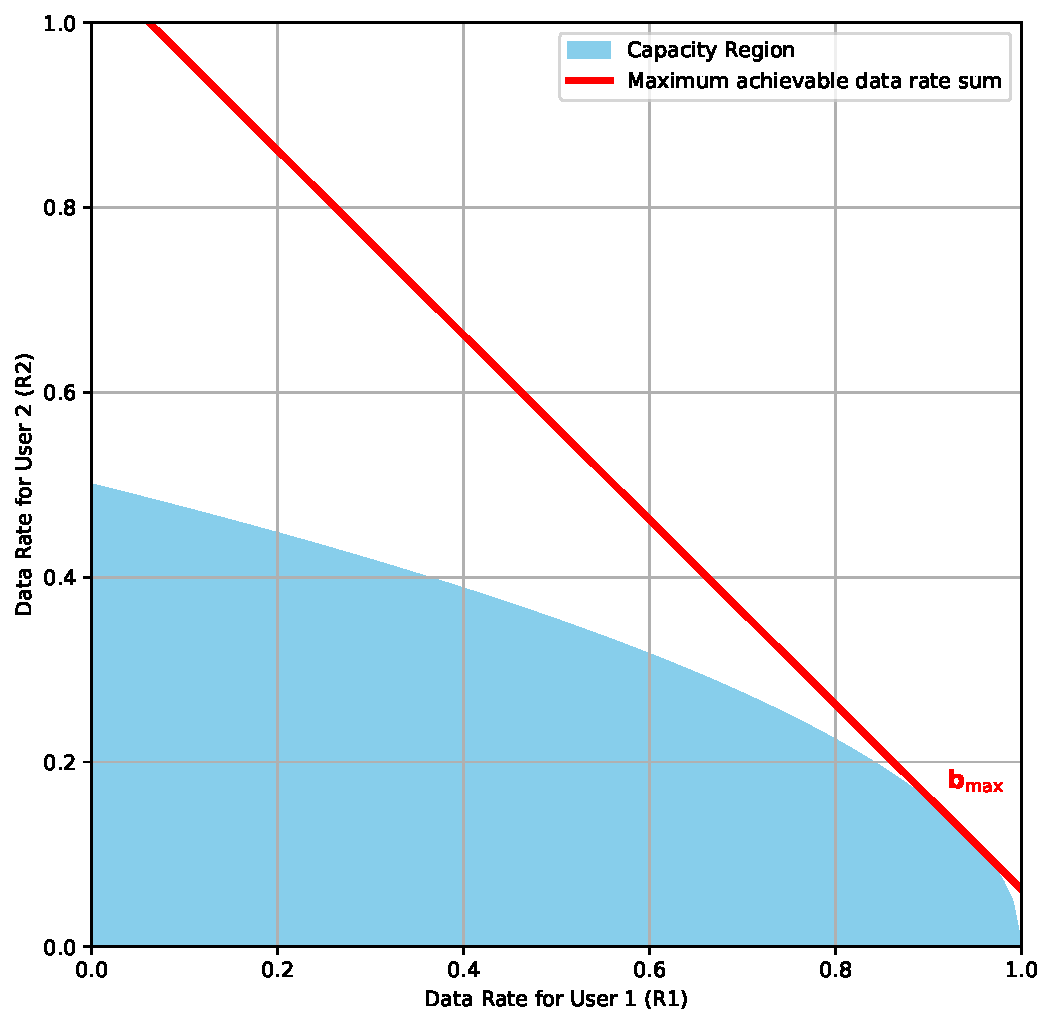
\includegraphics[width=6cm]{figures/Capacity_Region.pdf}
%     \caption{Capacity Region for two Users}
%     \label{fig:capacity_region}
% \end{figure}

% Repeat problem explanation
% Copy formulation from slides for energy minimization problem: explain and break it down into simpler subproblem by defining b, for example
% Explain GDFE from Chapter 5
% Explain minPMAC logic, ellipsoid, provide code from book , explain the concept of time sharing or vertex sharing
Generalized Decision-Feedback Equalizer (GDFE) has been proposed to resolve the issue of inter-symbol interference (ISI) in an AWGN channel. To achieve this, each symbol is detected based on all previously received symbols at the receiver\cite{yu2004sum}. In the case of a multiple-access channel, GDFE is utilized to eliminate interference caused by signals from other users on a specific user's signal.
% By assuming that the channel is non-singular, and we are using ideal code {\color{red} (Gap = 0)}, 

This paper compares the performance of non-linear (GDFE) receivers \cite{GDFE} {\color{red} Problem with Citation} and linear (OFDM) receivers\cite{chang1966synthesis}, focusing specifically on energy consumption. To begin, we will utilize the Simultaneous Water-Filling (SWF) algorithm\cite{book} with the linear receiver. This algorithm is designed to optimize the sum rate of data transmission within the constraints of available energy. Subsequently, we will use the GDFE approach in the receiver, targeting the data rate determined by the SWF algorithm to achieve energy minimization. Our objective is to demonstrate how effectively the energy requirements for the GDFE receiver can be reduced by leveraging the data rate values obtained from the SWF algorithm. {\color{red} why GDFE results in a better energy preservation?}

We adhere to the following notations throughout the paper. $U$ denotes the number of users. $\bar{N}$ represents the number of tones. $L_x$ and $L_y$ are the total number of the users' antennas and the total number of antennas at the access point, respectively. $L_{x,u}$ is the number of antennas for the $u^{th}$ user. Moreover, the subscripts $u$ and $n$ represent user $u$ and $n^{th}$ tone, respectively. For instance, $H_u$ represents the channel matrix for user $u$. 
% The duality between these two problems arises from their shared Lagrangian frameworks. Both problems involve a common Lagrangian term in their expressions, which indicates a zero duality gap for their respective optimizations under certain conditions. The Lagrangian expressions for both problems differ in how the parameters $\theta$ and $w$ are interpreted (as either given constants or Lagrange multipliers) and in the terms related to incremental change constraints.
Now, we will formulate two weighted-sum optimization problems: Energy Sum Minimization (\ref{Esum}) and Data Rate Sum Maximization (\ref{Rsum}).
\subsection{Energy Sum Minimization} \label{Esum}
The weighted Energy Sum Minimization is formulated as follows:
\begin{equation}
\begin{aligned}
\min_{\left\{R_{\boldsymbol{xx}}{(u)} \right\}} \quad & \sum_{u=1}^U w_u \cdot \operatorname{trace} \underbrace{\{R_{ \boldsymbol{x} \boldsymbol{x}}{(u)}\}}_{\mathcal{E}_u}\\
\textrm{s.t.} \quad & \mathbf{b} \succeq \left[b_{1, \min }, b_{2, \min }, \ldots, b_{U, \min }\right]^*\\
  &\mathcal{E}\geq0    \\
\end{aligned}
\end{equation}
Where $R_{\boldsymbol{xx}}(u)$ and $b_{u,\operatorname{min}}$ are the autocorrelation matrix and the minimum data rate required for the user $u$, respectively. Also, the vector $w \in \mathbb{R}_{0+}^U$ represents non-negative weights for each user's energy.

The corresponding Lagrangian function would be as follows:
% \begin{equation}
% \begin{aligned}
% \mathcal{L}\left(R_{\boldsymbol{x} \boldsymbol{x}}(n), \boldsymbol{b}, \boldsymbol{w}, \boldsymbol{\theta}\right)=\sum_{u=1}^U(&w_u \cdot\left[\sum_{n=0}^{\bar{N}} \operatorname{trace}\left\{R_{\boldsymbol{x} \boldsymbol{x}}(u, n)\right\}\right]+\\
% &\theta_u \cdot\left\{\left[\sum_{n=0}^{\bar{N}-1} b_{u, n}\right]-b_u\right\})
% \end{aligned}
% \end{equation}
\begin{equation}
\begin{aligned}
\mathcal{L}_{\min E}\left(R_{\boldsymbol{x} \boldsymbol{x}}, \boldsymbol{b}, \boldsymbol{w}, \boldsymbol{\theta}\right)=\max _{\boldsymbol{\theta}} \min _{R_{\boldsymbol{x} \boldsymbol{x}}} &\sum_{u=1}^U  w_u \cdot \operatorname{trace}\left\{R_{\boldsymbol{x} \boldsymbol{x}}(u)\right\}\\ &+ \theta_u \cdot b_u-\theta_u \cdot b_{\min , u}
\end{aligned}
\end{equation}
\subsection{Data Rate Sum Maximization} \label{Rsum}
The weighted Data Rate Sum Maximization problem can be formulated as follows:
\begin{equation}
\begin{aligned}
\max _{\left\{R_{\boldsymbol{x} \boldsymbol{x}}{(u)}\right\}} \quad &\sum_{u=1}^U \theta_u \cdot b_u \\
\textrm{s.t.} \quad &\mathcal{E}_{\boldsymbol{x}} \preceq\left[\mathcal{E}_{1,\max}, \mathcal{E}_{2,\text{max}},\ldots,\mathcal{E}_{U,\text{max}}\right]^*\\
& \mathbf{b} \succeq 0
\end{aligned}
\end{equation}
Similar to the previous part, we can expand the Lagrangian function:
\begin{equation}
\begin{aligned}
\mathcal{L}_{\max R}\left(R_{\boldsymbol{x} \boldsymbol{x}}, \boldsymbol{b}, \boldsymbol{w}, \boldsymbol{\theta}\right)=\min _{\boldsymbol{w}} \max _{R_{\boldsymbol{x} \boldsymbol{x}}} &\sum_{u=1}^U w_u \cdot \operatorname{trace}\left\{R_{\boldsymbol{x} \boldsymbol{x}}(u)\right\}\\ &+\:\theta_u \cdot b_u-w_u \cdot \mathcal{E}_{\max , u}
\end{aligned}
\end{equation} 

The common term $w_u \cdot \operatorname{trace}\left\{R_{\boldsymbol{x} \boldsymbol{x}}(u)\right\} + \theta_u \cdot b_u$ in both optimization problems implies the duality between them. Therefore, we will use a primal-dual approach to solve the optimization problem. In fact, we locate the optimal autocorrelation matrix $R_{\boldsymbol{xx}}$, while fulfilling both the data rate and energy constraints. 
% Both problems involve a common Lagrangian term in their expressions, which indicates a zero duality gap for their respective optimizations under certain conditions. The Lagrangian expressions for both problems differ in how the parameters $\theta$ and $w$ are interpreted (as either given constants or Lagrange multipliers) and in the terms related to incremental change constraints.



% As we can see, there is a common term in both optimization problems, and our algorithm tries to optimize these two problems simultaneously. Specifically, the algorithm locates the optimal $R_{\boldsymbol{xx}}$, while fulfilling both the data rate and energy constraints. 
It can be proven that the aforementioned optimization problems can be solved for each tone separately. In other words, an independent GDFE is assigned to each tone, and the total energy can be calculated by summing up all tones\cite{book}. The corresponding energy minimization problem for each tone is as follows:
\begin{equation} \label{tonalE}
    \begin{aligned}
        \min_{\left\{R_{\boldsymbol{x} \boldsymbol{x}}{(u, n)}\right\}} \quad &\sum_{u=1}^U \sum_{n=0}^{\bar{N}} w_u \cdot \operatorname{trace}\left\{R_{\boldsymbol{x} \boldsymbol{x}}(u, n)\right\} \\
        \textrm{s.t.} \quad &\mathbf{b}=\sum_{n=0}^{\bar{N}}\left[b_{1, n}, b_{2, n}, \ldots ,b_{U, n}\right]^* \succeq \boldsymbol{b}_{\min } \succeq \mathbf{0}
    \end{aligned}
\end{equation}
Where $R_{\boldsymbol{xx}}(u,n)\in\mathbb{R}^{L_{x,u}\times L_{x,u}}$ is the autocorrelation matrix of $\boldsymbol{x}$ for user $u$ on the $n^{th}$ tone. 

Similarly, the data rate maximization problem per each tone is expressed as:
\begin{equation}
\begin{aligned}
\max_{\left\{R_{\boldsymbol{x} \boldsymbol{x}}{(u, n)}\right\}} \quad &\sum_{u=1}^U \theta_u \cdot\left\{\sum_{n=0}^{\bar{N}} b_{u, n}\right\} \\
\textrm{s.t.} \quad &\mathcal{E}=\sum_{n=0}^{\bar{N}}\left[\mathcal{E}_{1, n}, \mathcal{E}_{2, n}, \ldots, \mathcal{E}_{U, n}\right]^* \preceq \boldsymbol{\mathcal{E}}_{\max }
\end{aligned}
\end{equation}
And the Lagrangian function for the equation \ref{tonalE} can be derived as follows:
\begin{equation} \label{minmaxE}
\begin{aligned}
\mathcal{L}_{\min E}\left(R_{\boldsymbol{x} \boldsymbol{x}}, \boldsymbol{b}, \boldsymbol{w}, \boldsymbol{\theta}\right)&=\left(\sum_{u=1}^U \theta_u \cdot b_u\right)
+ \\
& \hspace{-1.5cm} \sum_{n=0}^{\bar{N}-1}\{\underbrace{\sum_{u=1}^U\left[w_u \cdot \operatorname{trace}\left\{R_{\boldsymbol{x} \boldsymbol{x}}(u, n)\right\}-\theta_u \cdot b_{u, n}\right]}_{\mathcal{L}_n\left(R_{\boldsymbol{x} \boldsymbol{x}}(n), \boldsymbol{b}_n, \boldsymbol{w}, \boldsymbol{\theta}\right)}\}
\end{aligned}
\end{equation}
Where $R_{\boldsymbol{x} \boldsymbol{x}}(n)=\operatorname{blkdiag}\left\{R_{\boldsymbol{x} \boldsymbol{x}}(U, n), \ldots, R_{\boldsymbol{x} \boldsymbol{x}}(1, n)\right\}$, and the operator $\operatorname{blkdiag}$ aligns matrices along the diagonal of another matrix. The term $\mathcal{L}_n\left(R_{\boldsymbol{x} \boldsymbol{x}}(n), \boldsymbol{b}_n, \boldsymbol{w}, \boldsymbol{\theta}\right)$ is called the Tonal Lagrangian term. Since $\mathcal{L}_n$ does not depend on $b_u$, minimizing the tonal lagrangian term is synonymous with optimizing: 
\begin{equation}
\mathcal{L}_{\min E}(\boldsymbol{\theta}, n) \triangleq \min _{\left\{R_{\boldsymbol{xx}}(u, n), b_{u, n}\right\}} \mathcal{L}\left(R_{\boldsymbol{xx}}(n), \boldsymbol{b}_n, \boldsymbol{w}, \boldsymbol{\theta}\right)    
\end{equation}
Therefore, the min-max problem \ref{minmaxE} boils down to :
\begin{equation} \label{final}
\mathcal{L}_{\min E}^*=\max _{\boldsymbol{\theta}}\{\left[\sum_{n=0}^{\bar{N}-1} \mathcal{L}_{\min E}(\boldsymbol{\theta}, n)\right]+\hspace{-0.5cm}\underbrace{\sum_{u=1}^U \theta_u \cdot b_u}_{\text {independent of } R_{\boldsymbol{xx}}(u, n), n}\hspace{-0.5cm}\}
\end{equation}



Moreover, the data rates must lie in the capacity region defined by the system specifications. The capacity region, denoted as $\mathcal{C}(b)$, refers to the set of all possible rate vectors $b$ for users with independent messages, where each message is encoded using a code that achieves the single-user capacity. This set characterizes the rates at which all users can be reliably decoded with a negligible average error probability by a Maximum A Posteriori (MAP) detector or equivalently, a Maximum Likelihood (ML) detector with equally likely messages for all independent users. The capacity region is essentially the combination of rates at which the system can operate such that all users' messages are delivered correctly. %Figure \ref{fig:capacity_region} depicts the capacity region for two users. 
The capacity region can be derived based on the Shannon capacity formula as follows\cite{shannon}. 
\begin{equation}
0 \leq b_n %\sum_{\boldsymbol{u} \subseteq \boldsymbol{U}} b_{u, n}
\leq \log _2\left|\left(\sum_{u=1}^U \widetilde{H}_{u, n} \cdot R_{\boldsymbol{x} \boldsymbol{x}}(u, n) \cdot \widetilde{H}_{u, n}^*\right)+I\right|
\end{equation}

Where $\tilde{H}_{u, n}=R_{N N}^{-1 / 2}(n) \cdot H_{u, n}$ is the equivalent-white-noise channel per each tone. \\\\

% A multiple-input-multiple-output (MIMO) system with additive white Gaussian noise (AWGN) can be described as
% \begin{equation}
% \boldsymbol{y}=H \cdot \boldsymbol{x}+\boldsymbol{n}
% \end{equation}

% Where $H \in \mathbb{R}^{L_y \times L_x}$ is the channel matrix, and $x$, $y$ are the transmitted and received signals respectively. 
The inner part of the optimization problem \ref{final} ($\mathcal{L}_{\min E}(\boldsymbol{\theta}, n)$) can be solved using semi-definite programming (SDP), and the Ellipsoid method \cite{yudin1976constrained} {\color{red} Correct the citation part} is used for the outer part. 

If the channel matrix $H_{u,n}$ is non-singular and the system uses ideal codes ($\Gamma = 0 \textrm{dB}$), the ellipsoid method will converge to a unique optimal solution. In other words, the system assigns different dimensions, such as time and frequency, to each user separately. However, if the channel is singular, the Hessian matrix computed at each iteration of the ellipsoid method will be degraded, and the optimization problem will not have a unique minimizer. In this case, the algorithm allows more than one user to use some specific dimensions at the same time, which is known as “time-sharing”. When the users “time-share” with one another, the algorithm cannot evaluate their individual optimal data rate, and it is only capable of computing the weighted sum of their data rates.  

% If the optimal point of energy lies inside the capacity-energy region, the Ellipsoid algorithm can find this point successfully. However, as we get closer to the boundary of the capacity region, the Hessian matrix constructed in the Ellipsoid algorithm will become singular (the minimum eigenvalue of the Hessian matrix will get closer to zero). Under these conditions, the system is stressed, making it more challenging for the Ellipsoid method to converge.

% {\color{red}this paragraph or above} Our algorithm is capable of stressing the system as much as possible so that each user doesn't experience low data rate. However, this goal is within reach only by using time-sharing, which is synonymous with allowing users to use the same amount of resources at the same time.

Finally, the minPMAC algorithm can be seen in algorithm 2. At first, we use the SWF algorithm to get an initialization for the ellipsoid parameters. Then, we are alternating between two optimization problems until convergence. It is worth mentioning that we prioritize the users' decoding process based on $\theta$ at each iteration.

% \begin{table}[t]
%     \caption{Notation Explanation}
%     \centering
%     \begin{tabular}{|c|c|}
%     \hline
%        \textbf{Parameter}  &  \textbf{Explanation}\\ \hline
%        $U$ & Number of users\\ 
%        $N$ & Number of tones\\
%        $L_x$ & Total number of users' antennas\\
%        $L_y$ & Total number of antennas at the access point\\ 
%        $L_{x,u}$ & user $u^{th}$ number of  antennas \\  \hline
        
%     \end{tabular}
%     \label{tab:ranging-imu-params}
% \end{table}



\begin{algorithm}[t]
	\caption{SWF} 
	% \begin{algorithmic}[1]
    \State \textbf{Inputs:} $H, L_x, R_{nn}$
		\For {$u=1,2,\ldots,U$}
            \State $R_{\text {noise}}(u) \triangleq \sum_{i \neq u} H_i \cdot R_{\boldsymbol{x} \boldsymbol{x}}(i) \cdot H_i^*+R_{\boldsymbol{nn}}$
            \vspace{0.1cm}\State $R_{\text {noise }}^{-1 / 2}(u) \cdot H_u=F_u \cdot \Lambda_u \cdot M_u^*$
            \vspace{0.1cm}\For{$\ell = 1,2,\ldots, L_x$}
                \State $\mathcal{E}_{u,\ell} = \operatorname{max} \left\{0, {\frac{1}{L_x}}\left(\mathcal{E}_u - \sum_{k=1}^{L_x}\frac{1}{\lambda_{u,k}^2}\right) - \frac{1}{\lambda_{u,\ell}^2}\right\}$
            \vspace{0.1cm}\EndFor
		\EndFor
\State \textbf{return} $\mathcal{E}_u$
\end{algorithm}

\begin{algorithm}[t]
	\caption{minPMAC} 
	% \begin{algorithmic}[1]
    \State \textbf{Inputs:} $H$, $L_{xu}$, $b_u$, $w$ 
    \vspace{0.1cm}
    \State \textbf{Initialize:} $A$, $\theta$ using SWF
    % \vspace{0.1cm}
    % \State $Idx_{END} = \operatorname{cumsum}(L_{xu})$
    % \vspace{0.1cm}
    % \State $Idx_{START} = [1, Idx_{END}(1:end-1)+1]$ 
    % \vspace{0.1cm}
    % \State $D \in \mathbb{R}^{U\times U}, \quad D_{i,i} = 1, D_{i,i+1} = -1 \quad \forall 1\leq i \leq U-1$
    % \vspace{0.1cm}
    \While {the sum rate doesn't converge}
    \vspace{0.1cm}
    \State $\pi \triangleq$ Indices of sorted $\theta$ in descending order
    \vspace{0.1cm}
       \For {$n = 1,2, \ldots,\bar{N}$}
        \vspace{0.1cm}
            \For{$u = 1,2,\ldots,U$}
                \vspace{0.1cm}
                \State \hspace{-0.3cm} $\footnotesize \mathcal{E}_{u,n} = \operatorname{trace}\left(R_{\boldsymbol{x} \boldsymbol{x}}\left(\pi^{-1}(u), n\right)\right)$
                \vspace{0.1cm}
                \State \hspace{-0.3cm} $\footnotesize \mathcal{R}_{u,n} \triangleq  \log _2\left|\sum_{i=u}^U \tilde{H}_{\pi^{-1}(i), n} \cdot R_{\boldsymbol{x} \boldsymbol{x}}\left(\pi^{-1}(i), n\right) \cdot \tilde{H}_{\pi^{-1}(i), n}^*+I\right|$
            \EndFor 
            \vspace{-0.7cm}
            \State \begin{equation*}
            \hspace{0.7cm} b_{u,n}^*=\underset{{R_{\boldsymbol{xx}}}}{\operatorname{argmin}} \quad \sum_{u=1}^U w_{u} \cdot \: \mathcal{E}_{u,n}- \left(\theta_{\pi^{-1}(u)}-\theta_{\pi^{-1}(u+1)}\right) \cdot \: \mathcal{R}_{u,n} \end{equation*}
            \vspace{-0.6cm}
            \State \begin{equation*}
                \hspace{-1.6cm} \textrm{s.t.} \quad R_{\boldsymbol{xx}}  \succeq \mathbf{0}
            \end{equation*}
    \EndFor 
    \vspace{0.1cm}
    \State $g = \sum_{n = 1}^{\bar{N}}  b_{u,n}^* - b_u$
    \vspace{0.1cm}
	\State $\tilde{g} = \frac{1}{\sqrt[]{g^TAg}}g$
    \vspace{0.1cm}
    \State $\theta = \theta - \frac{1}{U+1}\frac{Ag}{\sqrt[]{g^TAg}}$
    \vspace{0.1cm}
    \State $A = \frac{U^2}{U^2-1}(A - \frac{2}{U+1} A \tilde{g}\tilde{g}^T A)$
    % \vspace{0.1cm}
    % \State $\mathcal{S} = \left\{i \: | \: \theta_i < 0\right\}$
    % \vspace{0.1cm}
    % \While {$\mathcal{S} \neq \left\{\right\}$}
    %     \State $g = \mathbf{0}$
    %     \vspace{0.1cm}
    %     \State $g(\mathcal{S}(1)) = 1$
    %     \vspace{0.1cm}
    % 	\State $\tilde{g} = \frac{1}{\sqrt[]{g^TAg}}g$
    %     \vspace{0.1cm}
    %     \State $\theta = \theta - \frac{1}{U+1}\frac{Ag}{\sqrt[]{g^TAg}}$
    %     \vspace{0.1cm}
    %     \State $A = \frac{U^2}{U^2-1}(A - \frac{2}{U+1} A \tilde{g}\tilde{g}^T A)$
    %     \vspace{0.1cm}
    %     \State $\mathcal{S} = \left\{i \: | \: \theta_i < 0\right\}$
    % \ENDWHILE
\ENDWHILE
\vspace{0.1cm}
\State \textbf{return} $b_{u,n}^*, \: \mathcal{E}_{u,n}$
\end{algorithm}

% \section{Methodology}
\begin{figure}
    \centering
    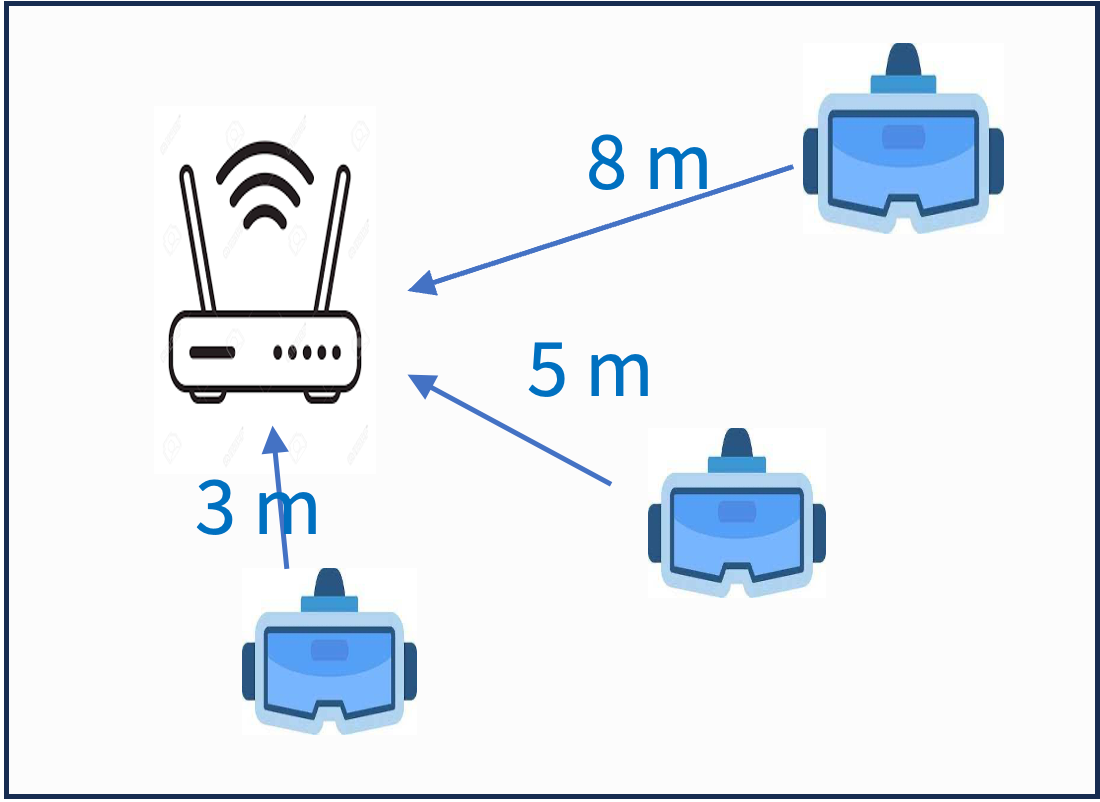
\includegraphics{figures/xr.png}
    \caption{XR Scenario: Distributed Rendering using VR glasses}
    \label{fig:xr}
\end{figure}
% \begin{figure}
%     \centering
%     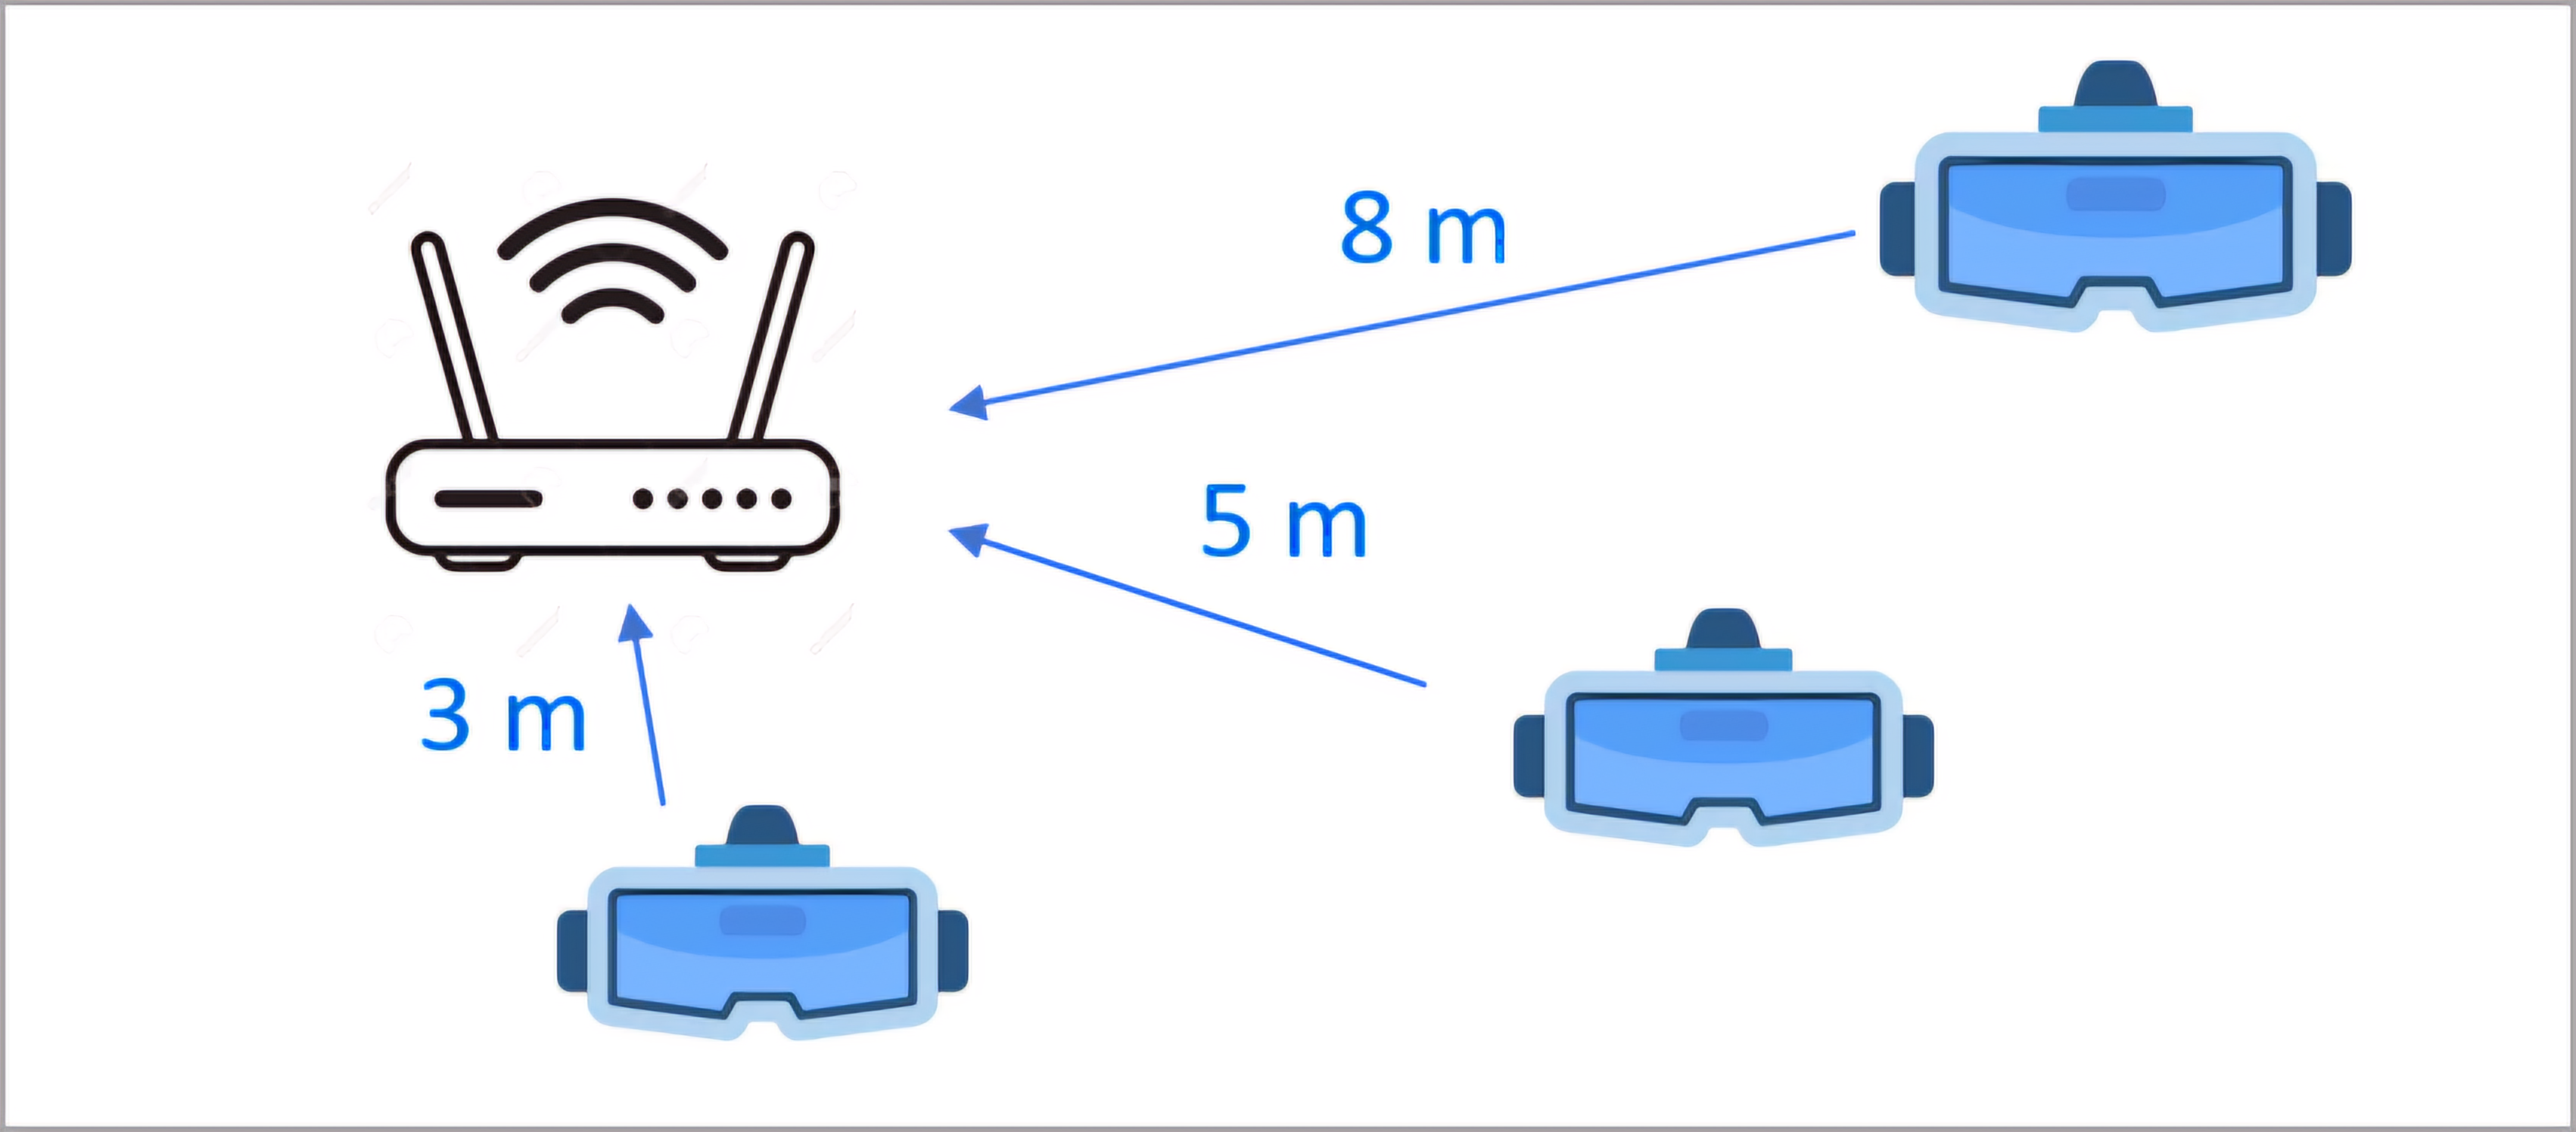
\includegraphics{figures/3_5_8_scenario.pdf}
%     \caption{XR Scenario: Distributed Rendering using VR glasses}
%     \label{fig:xr}
% \end{figure}


% \begin{figure}
%     \centering
%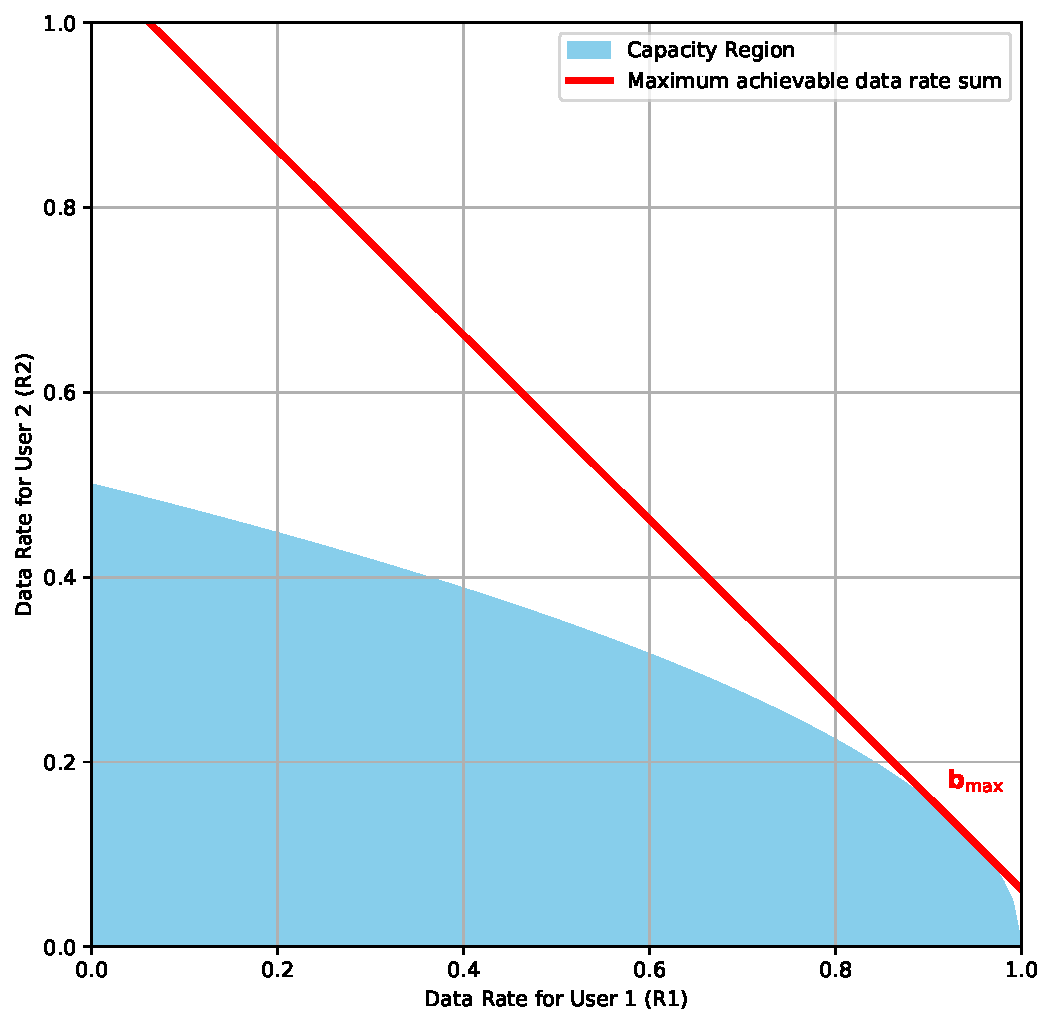
\includegraphics[width=6cm]{figures/Capacity_Region.pdf}
%     \caption{Capacity Region for two Users}
%     \label{fig:capacity_region}
% \end{figure}
% Repeat problem explanation
% Copy formulation from slides for energy minimization problem: explain and break it down into simpler subproblem by defining b, for example
% Explain GDFE from Chapter 5
% Explain minPMAC logic, ellipsoid, provide code from book , explain the concept of time sharing or vertex sharing
The Generalized Decision-Feedback Equalizer (GDFE) resolves multiuser crosstalk issues. To achieve this, each users data is detected based on all previously decoded users with each symbol \cite{yu2004sum}, \cite{book}. % By assuming that the channel is non-singular, and we are using ideal code {\color{red} (Gap = 0)}, 

This work compares the performance of non-linear (GDFE) receivers \cite{GDFE} {\color{red} Problem with Citation} and linear receivers\cite{chang1966synthesis}, both using basic OFDM.  The specific focus is energy consumption. Initially, the receiver analysis uses the Simultaneous Water-Filling (SWF) algorithm\cite{book} with the linear receiver.  This SWF optimizes the sum data rate for a given available energy. Subsequently, a receiver uses the GDFE, targeting the data rate determined by the SWF algorithm, to minimize energy. The objective is to demonstrate how the GDFE receiver can substantially reduce energy consumption in attaining the same SWF data rate values obtained. {\color{red} why GDFE results in a better energy preservation?}

Notation includes: $U$ denotes the number of users. $\bar{N}$ represents the number of tones. $L_x$ and $L_y$ are the total number of users' antennas and the total number of antennas at the access point, respectively. $L_{x,u}$ is the number of antennas for the $u^{th}$ user. Moreover, the subscripts $u$ and $n$ represent user $u$ and $n^{th}$ tone, respectively. For instance, $H_u$ is user $u$'s channel matrix. 
% The duality between these two problems arises from their shared Lagrangian frameworks. Both problems involve a common Lagrangian term in their expressions, which indicates a zero duality gap for their respective optimizations under certain conditions. The Lagrangian expressions for both problems differ in how the parameters $\theta$ and $w$ are interpreted (as either given constants or Lagrange multipliers) and in the terms related to incremental change constraints.
There are two weighted-sum optimization problems: Energy Sum Minimization (\ref{Esum}) and Data Rate Sum Maximization (\ref{Rsum}).
\subsection{Energy Sum Minimization} \label{Esum}
The weighted Energy Sum Minimization is formulated as follows:
\begin{equation}
\begin{aligned}
\min_{\left\{R_{\boldsymbol{xx}}{(u)} \right\}} \quad & \sum_{u=1}^U w_u \cdot \operatorname{trace} \underbrace{\{R_{ \boldsymbol{x} \boldsymbol{x}}{(u)}\}}_{\mathcal{E}_u}\\
\textrm{s.t.} \quad & \mathbf{b} \succeq \left[b_{1, \min }, b_{2, \min }, \ldots, b_{U, \min }\right]^*\\
  &\mathcal{E}\geq0    \\
\end{aligned}
\end{equation}
Where $R_{\boldsymbol{xx}}(u)$ and $b_{u,\operatorname{min}}$ are the autocorrelation matrix and user $u$'s minimum data rate, respectively. Also, the vector $w \in \mathbb{R}_{0+}^U$ represents non-negative weights for each user's energy.

The corresponding Lagrangian function is:
% \begin{equation}
% \begin{aligned}
% \mathcal{L}\left(R_{\boldsymbol{x} \boldsymbol{x}}(n), \boldsymbol{b}, \boldsymbol{w}, \boldsymbol{\theta}\right)=\sum_{u=1}^U(&w_u \cdot\left[\sum_{n=0}^{\bar{N}} \operatorname{trace}\left\{R_{\boldsymbol{x} \boldsymbol{x}}(u, n)\right\}\right]+\\
% &\theta_u \cdot\left\{\left[\sum_{n=0}^{\bar{N}-1} b_{u, n}\right]-b_u\right\})
% \end{aligned}
% \end{equation}
\begin{equation}
\begin{aligned}
\mathcal{L}_{\min E}\left(R_{\boldsymbol{x} \boldsymbol{x}}, \boldsymbol{b}, \boldsymbol{w}, \boldsymbol{\theta}\right)=\max _{\boldsymbol{\theta}} \min _{R_{\boldsymbol{x} \boldsymbol{x}}} &\sum_{u=1}^U  w_u \cdot \operatorname{trace}\left\{R_{\boldsymbol{x} \boldsymbol{x}}(u)\right\}\\ &+ \theta_u \cdot b_u-\theta_u \cdot b_{\min , u}
\end{aligned}
\end{equation}
\subsection{Data Rate Sum Maximization} \label{Rsum}
The weighted Data Rate Sum Maximization problem can be formulated as follows:
\begin{equation}
\begin{aligned}
\max _{\left\{R_{\boldsymbol{x} \boldsymbol{x}}{(u)}\right\}} \quad &\sum_{u=1}^U \theta_u \cdot b_u \\
\textrm{s.t.} \quad &\mathcal{E}_{\boldsymbol{x}} \preceq\left[\mathcal{E}_{1,\max}, \mathcal{E}_{2,\text{max}},\ldots,\mathcal{E}_{U,\text{max}}\right]^*\\
& \mathbf{b} \succeq 0
\end{aligned}
\end{equation}
Similar to the previous part, we can expand the Lagrangian function:
\begin{equation}
\begin{aligned}
\mathcal{L}_{\max R}\left(R_{\boldsymbol{x} \boldsymbol{x}}, \boldsymbol{b}, \boldsymbol{w}, \boldsymbol{\theta}\right)=\min _{\boldsymbol{w}} \max _{R_{\boldsymbol{x} \boldsymbol{x}}} &\sum_{u=1}^U w_u \cdot \operatorname{trace}\left\{R_{\boldsymbol{x} \boldsymbol{x}}(u)\right\}\\ &+\:\theta_u \cdot b_u-w_u \cdot \mathcal{E}_{\max , u}
\end{aligned}
\end{equation} 

The common term $w_u \cdot \operatorname{trace}\left\{R_{\boldsymbol{x} \boldsymbol{x}}(u)\right\} + \theta_u \cdot b_u$ in both optimization problems implies their duality. Therefore, a primal-dual approach solves the optimization problem.This locates the optimal autocorrelation matrix $R_{\boldsymbol{xx}}$, while fulfilling both the data rate and energy constraints. 
% Both problems involve a common Lagrangian term in their expressions, which indicates a zero duality gap for their respective optimizations under certain conditions. The Lagrangian expressions for both problems differ in how the parameters $\theta$ and $w$ are interpreted (as either given constants or Lagrange multipliers) and in the terms related to incremental change constraints.


% As we can see, there is a common term in both optimization problems, and our algorithm tries to optimize these two problems simultaneously. Specifically, the algorithm locates the optimal $R_{\boldsymbol{xx}}$, while fulfilling both the data rate and energy constraints. 
It can be proven that the aforementioned optimization problems can be solved for each tone separately. In other words, an independent GDFE is assigned to each tone, and the total energy can be calculated by summing up all tones\cite{book}. The corresponding energy minimization problem for each tone is as follows:
\begin{equation} \label{tonalE}
    \begin{aligned}
        \min_{\left\{R_{\boldsymbol{x} \boldsymbol{x}}{(u, n)}\right\}} \quad &\sum_{u=1}^U \sum_{n=0}^{\bar{N}} w_u \cdot \operatorname{trace}\left\{R_{\boldsymbol{x} \boldsymbol{x}}(u, n)\right\} \\
        \textrm{s.t.} \quad &\mathbf{b}=\sum_{n=0}^{\bar{N}}\left[b_{1, n}, b_{2, n}, \ldots ,b_{U, n}\right]^* \succeq \boldsymbol{b}_{\min } \succeq \mathbf{0}
    \end{aligned}
\end{equation}
Where $R_{\boldsymbol{xx}}(u,n)\in\mathbb{R}^{L_{x,u}\times L_{x,u}}$ is the autocorrelation matrix of $\boldsymbol{x}$ for user $u$ on the $n^{th}$ tone. 

Similarly, the data rate maximization problem per each tone is:
\begin{equation}
\begin{aligned}
\max_{\left\{R_{\boldsymbol{x} \boldsymbol{x}}{(u, n)}\right\}} \quad &\sum_{u=1}^U \theta_u \cdot\left\{\sum_{n=0}^{\bar{N}} b_{u, n}\right\} \\
\textrm{s.t.} \quad &\mathcal{E}=\sum_{n=0}^{\bar{N}}\left[\mathcal{E}_{1, n}, \mathcal{E}_{2, n}, \ldots, \mathcal{E}_{U, n}\right]^* \preceq \boldsymbol{\mathcal{E}}_{\max } \;\;.
\end{aligned}
\end{equation}
Equation \ref{tonalE} 's Lagrangian function is:
\begin{equation} \label{minmaxE}
\begin{aligned}
\mathcal{L}_{\min E}\left(R_{\boldsymbol{x} \boldsymbol{x}}, \boldsymbol{b}, \boldsymbol{w}, \boldsymbol{\theta}\right)&=\left(\sum_{u=1}^U \theta_u \cdot b_u\right)
+ \\
& \hspace{-1.5cm} \sum_{n=0}^{\bar{N}-1}\{\underbrace{\sum_{u=1}^U\left[w_u \cdot \operatorname{trace}\left\{R_{\boldsymbol{x} \boldsymbol{x}}(u, n)\right\}-\theta_u \cdot b_{u, n}\right]}_{\mathcal{L}_n\left(R_{\boldsymbol{x} \boldsymbol{x}}(n), \boldsymbol{b}_n, \boldsymbol{w}, \boldsymbol{\theta}\right)}\}
\end{aligned}
\end{equation}
Where $R_{\boldsymbol{x} \boldsymbol{x}}(n)=\operatorname{blkdiag}\left\{R_{\boldsymbol{x} \boldsymbol{x}}(U, n), \ldots, R_{\boldsymbol{x} \boldsymbol{x}}(1, n)\right\}$, and the operator $\operatorname{blkdiag}$ aligns matrices along the diagonal of another matrix. The term $\mathcal{L}_n\left(R_{\boldsymbol{x} \boldsymbol{x}}(n), \boldsymbol{b}_n, \boldsymbol{w}, \boldsymbol{\theta}\right)$ is called the Tonal Lagrangian term. Since $\mathcal{L}_n$ does not depend on $b_u$, minimizing the tonal lagrangian term is synonymous with optimizing: 
\begin{equation}
\mathcal{L}_{\min E}(\boldsymbol{\theta}, n) \triangleq \min _{\left\{R_{\boldsymbol{xx}}(u, n), b_{u, n}\right\}} \mathcal{L}\left(R_{\boldsymbol{xx}}(n), \boldsymbol{b}_n, \boldsymbol{w}, \boldsymbol{\theta}\right)    
\end{equation}
Therefore, the min-max problem \ref{minmaxE} reduces to :
\begin{equation} \label{final}
\mathcal{L}_{\min E}^*=\max _{\boldsymbol{\theta}}\{\left[\sum_{n=0}^{\bar{N}-1} \mathcal{L}_{\min E}(\boldsymbol{\theta}, n)\right]+\hspace{-0.5cm}\underbrace{\sum_{u=1}^U \theta_u \cdot b_u}_{\text {independent of } R_{\boldsymbol{xx}}(u, n), n}\hspace{-0.5cm}\}
\end{equation}

Moreover, the data rates must lie in the system's capacity region. The capacity region, denoted as $\mathcal{C}(b)$, refers to the set of all possible rate vectors $b$ for users with independent messages, where each message employs a code that achieves the single-user capacity. This code is used for all systems and differences in their performance therefore solely derives from the GDFE improvement over the linear receiver.  This set characterizes the rates at which all users can be reliably decoded with a negligible average error probability by a Maximum A Posteriori (MAP) detector or equivalently, a Maximum Likelihood (ML) detector with equally likely messages for all independent users. The capacity region is essentially the combination of rates at which the system can operate such that all users' messages are delivered correctly. %Figure \ref{fig:capacity_region} depicts the capacity region for two users. 
The capacity region follows from the Shannon capacity formula as \cite{shannon}: 
\begin{equation}
0 \leq b_n %\sum_{\boldsymbol{u} \subseteq \boldsymbol{U}} b_{u, n}
\leq \log _2\left|\left(\sum_{u=1}^U \widetilde{H}_{u, n} \cdot R_{\boldsymbol{x} \boldsymbol{x}}(u, n) \cdot \widetilde{H}_{u, n}^*\right)+I\right|
\end{equation}

$\tilde{H}_{u, n}=R_{N N}^{-1 / 2}(n) \cdot H_{u, n}$ is the equivalent-white-noise channel per each tone.
% A multiple-input-multiple-output (MIMO) system with additive white Gaussian noise (AWGN) can be described as
% \begin{equation}
% \boldsymbol{y}=H \cdot \boldsymbol{x}+\boldsymbol{n}
% \end{equation}

% Where $H \in \mathbb{R}^{L_y \times L_x}$ is the channel matrix, and $x$, $y$ are the transmitted and received signals respectively. 
A semi-definite programming (SDP) method solves the inner optimization problem \ref{final} ($\mathcal{L}_{\min E}(\boldsymbol{\theta}, n)$), while an Ellipsoid method \cite{yudin1976constrained} {\color{red} Correct the citation part} optimizes the outer part. 
If the channel matrix $H_{u,n}$ is non-singular with the ideal common codes mentioned ($\Gamma = 0 \textrm{dB}$), the ellipsoid method finds a unique optimal solution. In other words, the system assigns different dimensions, such as time and frequency, to each user separately. However, if the channel is singular, the Hessian matrix computed at each ellipsoid-method iteration degradeds, and the optimization problem does not have a unique solution. In this case, the algorithm allows more than one user to use some specific dimensions at the same time, which is known as “time-sharing”. When the users “time-share” with one another, the algorithm only finds the weighted sum.  A separate time-sharing step then applies to ensure all users meet their target data rate.  

% If the optimal point of energy lies inside the capacity-energy region, the Ellipsoid algorithm can find this point successfully. However, as we get closer to the boundary of the capacity region, the Hessian matrix constructed in the Ellipsoid algorithm will become singular (the minimum eigenvalue of the Hessian matrix will get closer to zero). Under these conditions, the system is stressed, making it more challenging for the Ellipsoid method to converge.

% {\color{red}this paragraph or above} Our algorithm is capable of stressing the system as much as possible so that each user doesn't experience low data rate. However, this goal is within reach only by using time-sharing, which is synonymous with allowing users to use the same amount of resources at the same time.

This minPMAC algorithm appears as Algorithm 2.  Initially, the SWF algorithm provides first ellipsoid parameters. Then, minPMAC alternates between two optimization problems until convergence. It prioritizes the users' decoding process based on $\theta$ at each iteration.

% \begin{table}[t]
%     \caption{Notation Explanation}
%     \centering
%     \begin{tabular}{|c|c|}
%     \hline
%        \textbf{Parameter}  &  \textbf{Explanation}\\ \hline
%        $U$ & Number of users\\ 
%        $N$ & Number of tones\\
%        $L_x$ & Total number of users' antennas\\
%        $L_y$ & Total number of antennas at the access point\\ 
%        $L_{x,u}$ & user $u^{th}$ number of  antennas \\  \hline
        
%     \end{tabular}
%     \label{tab:ranging-imu-params}
% \end{table}



\begin{algorithm}[t]
	\caption{SWF} 
	% \begin{algorithmic}[1]
    \State \textbf{Inputs:} $H, L_x, R_{nn}$
		\For {$u=1,2,\ldots,U$}
            \State $R_{\text {noise}}(u) \triangleq \sum_{i \neq u} H_i \cdot R_{\boldsymbol{x} \boldsymbol{x}}(i) \cdot H_i^*+R_{\boldsymbol{nn}}$
            \vspace{0.1cm}\State $R_{\text {noise }}^{-1 / 2}(u) \cdot H_u=F_u \cdot \Lambda_u \cdot M_u^*$
            \vspace{0.1cm}\For{$\ell = 1,2,\ldots, L_x$}
                \State $\mathcal{E}_{u,\ell} = \operatorname{max} \left\{0, {\frac{1}{L_x}}\left(\mathcal{E}_u - \sum_{k=1}^{L_x}\frac{1}{\lambda_{u,k}^2}\right) - \frac{1}{\lambda_{u,\ell}^2}\right\}$
            \vspace{0.1cm}\EndFor
		\EndFor
\State \textbf{return} $\mathcal{E}_u$
\end{algorithm}

\begin{algorithm}[t]
	\caption{minPMAC} 
	% \begin{algorithmic}[1]
    \State \textbf{Inputs:} $H$, $L_{xu}$, $b_u$, $w$ 
    \vspace{0.1cm}
    \State \textbf{Initialize:} $A$, $\theta$ using SWF
    % \vspace{0.1cm}
    % \State $Idx_{END} = \operatorname{cumsum}(L_{xu})$
    % \vspace{0.1cm}
    % \State $Idx_{START} = [1, Idx_{END}(1:end-1)+1]$ 
    % \vspace{0.1cm}
    % \State $D \in \mathbb{R}^{U\times U}, \quad D_{i,i} = 1, D_{i,i+1} = -1 \quad \forall 1\leq i \leq U-1$
    % \vspace{0.1cm}
    \While {the sum rate doesn't converge}
    \vspace{0.1cm}
    \State $\pi \triangleq$ Indices of sorted $\theta$ in descending order
    \vspace{0.1cm}
       \For {$n = 1,2, \ldots,\bar{N}$}
        \vspace{0.1cm}
            \For{$u = 1,2,\ldots,U$}
                \vspace{0.1cm}
                \State \hspace{-0.3cm} $\footnotesize \mathcal{E}_{u,n} = \operatorname{trace}\left(R_{\boldsymbol{x} \boldsymbol{x}}\left(\pi^{-1}(u), n\right)\right)$
                \vspace{0.1cm}
                \State \hspace{-0.3cm} $\footnotesize \mathcal{R}_{u,n} \triangleq  \log _2\left|\sum_{i=u}^U \tilde{H}_{\pi^{-1}(i), n} \cdot R_{\boldsymbol{x} \boldsymbol{x}}\left(\pi^{-1}(i), n\right) \cdot \tilde{H}_{\pi^{-1}(i), n}^*+I\right|$
            \EndFor 
            \vspace{-0.7cm}
            \State \begin{equation*}
            \hspace{0.7cm} b_{u,n}^*=\underset{{R_{\boldsymbol{xx}}}}{\operatorname{argmin}} \quad \sum_{u=1}^U w_{u} \cdot \: \mathcal{E}_{u,n}- \left(\theta_{\pi^{-1}(u)}-\theta_{\pi^{-1}(u+1)}\right) \cdot \: \mathcal{R}_{u,n} \end{equation*}
            \vspace{-0.6cm}
            \State \begin{equation*}
                \hspace{-1.6cm} \textrm{s.t.} \quad R_{\boldsymbol{xx}}  \succeq \mathbf{0}
            \end{equation*}
    \EndFor 
    \vspace{0.1cm}
    \State $g = \sum_{n = 1}^{\bar{N}}  b_{u,n}^* - b_u$
    \vspace{0.1cm}
	\State $\tilde{g} = \frac{1}{\sqrt[]{g^TAg}}g$
    \vspace{0.1cm}
    \State $\theta = \theta - \frac{1}{U+1}\frac{Ag}{\sqrt[]{g^TAg}}$
    \vspace{0.1cm}
    \State $A = \frac{U^2}{U^2-1}(A - \frac{2}{U+1} A \tilde{g}\tilde{g}^T A)$
    % \vspace{0.1cm}
    % \State $\mathcal{S} = \left\{i \: | \: \theta_i < 0\right\}$
    % \vspace{0.1cm}
    % \While {$\mathcal{S} \neq \left\{\right\}$}
    %     \State $g = \mathbf{0}$
    %     \vspace{0.1cm}
    %     \State $g(\mathcal{S}(1)) = 1$
    %     \vspace{0.1cm}
    % 	\State $\tilde{g} = \frac{1}{\sqrt[]{g^TAg}}g$
    %     \vspace{0.1cm}
    %     \State $\theta = \theta - \frac{1}{U+1}\frac{Ag}{\sqrt[]{g^TAg}}$
    %     \vspace{0.1cm}
    %     \State $A = \frac{U^2}{U^2-1}(A - \frac{2}{U+1} A \tilde{g}\tilde{g}^T A)$
    %     \vspace{0.1cm}
    %     \State $\mathcal{S} = \left\{i \: | \: \theta_i < 0\right\}$
    % \ENDWHILE
\ENDWHILE
\vspace{0.1cm}
\State \textbf{return} $b_{u,n}^*, \: \mathcal{E}_{u,n}$
\end{algorithm}

\section{Methodology}

\begin{figure}
    \centering
    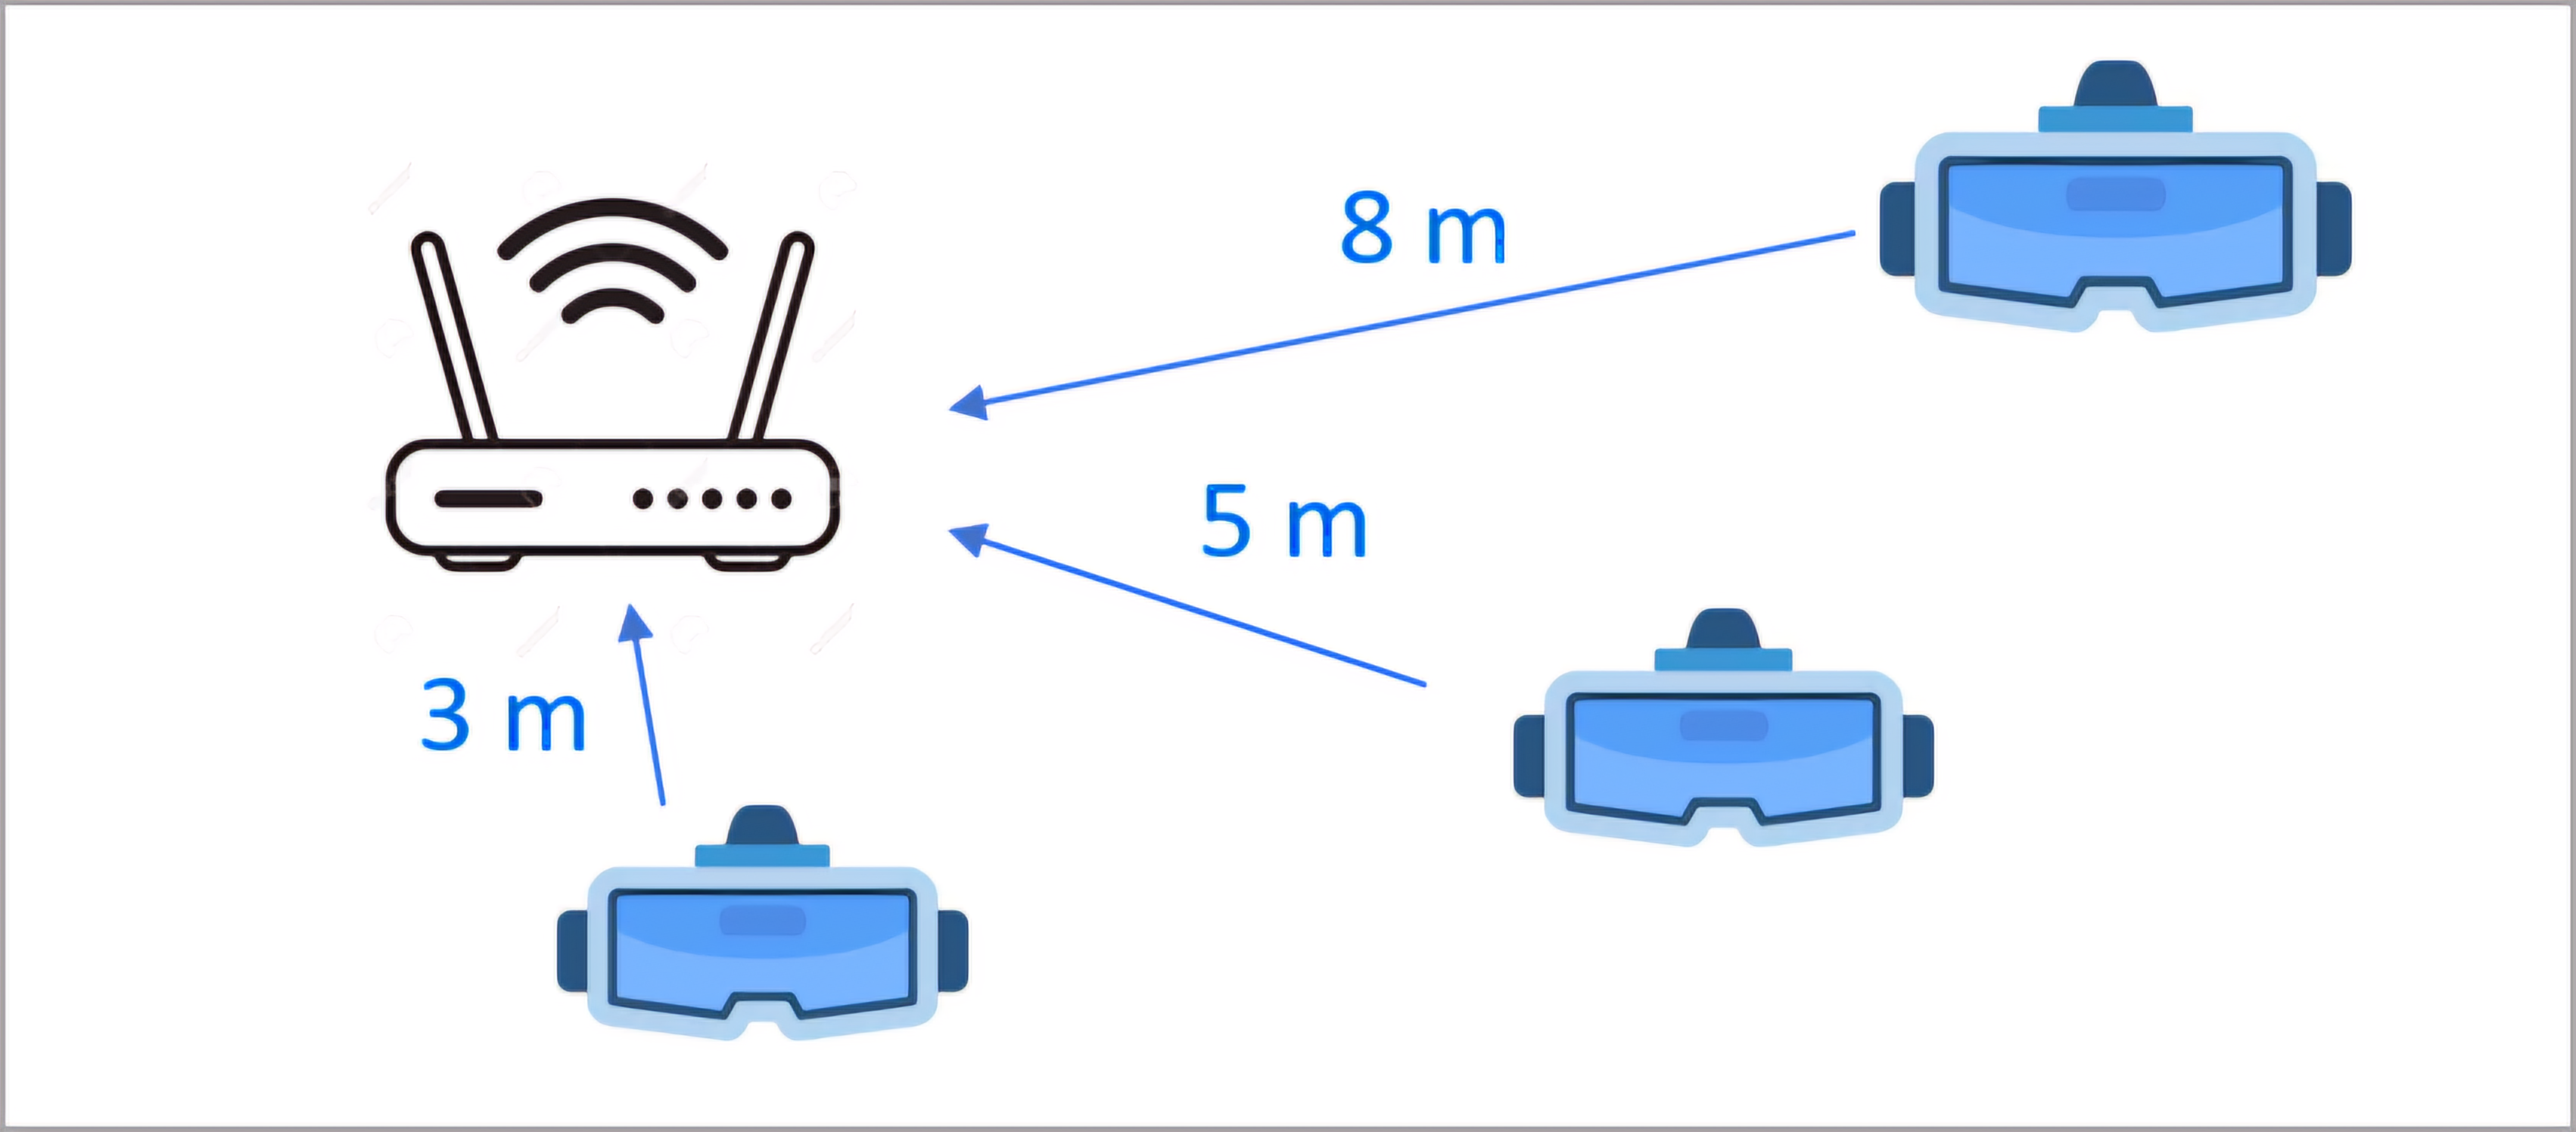
\includegraphics[width=0.48\textwidth, height=4.8cm]{figures/3_5_8_scenario.png}
    \caption{XR Scenario}
    \label{fig:xr}
\end{figure}
% \begin{figure}
%     \centering
%     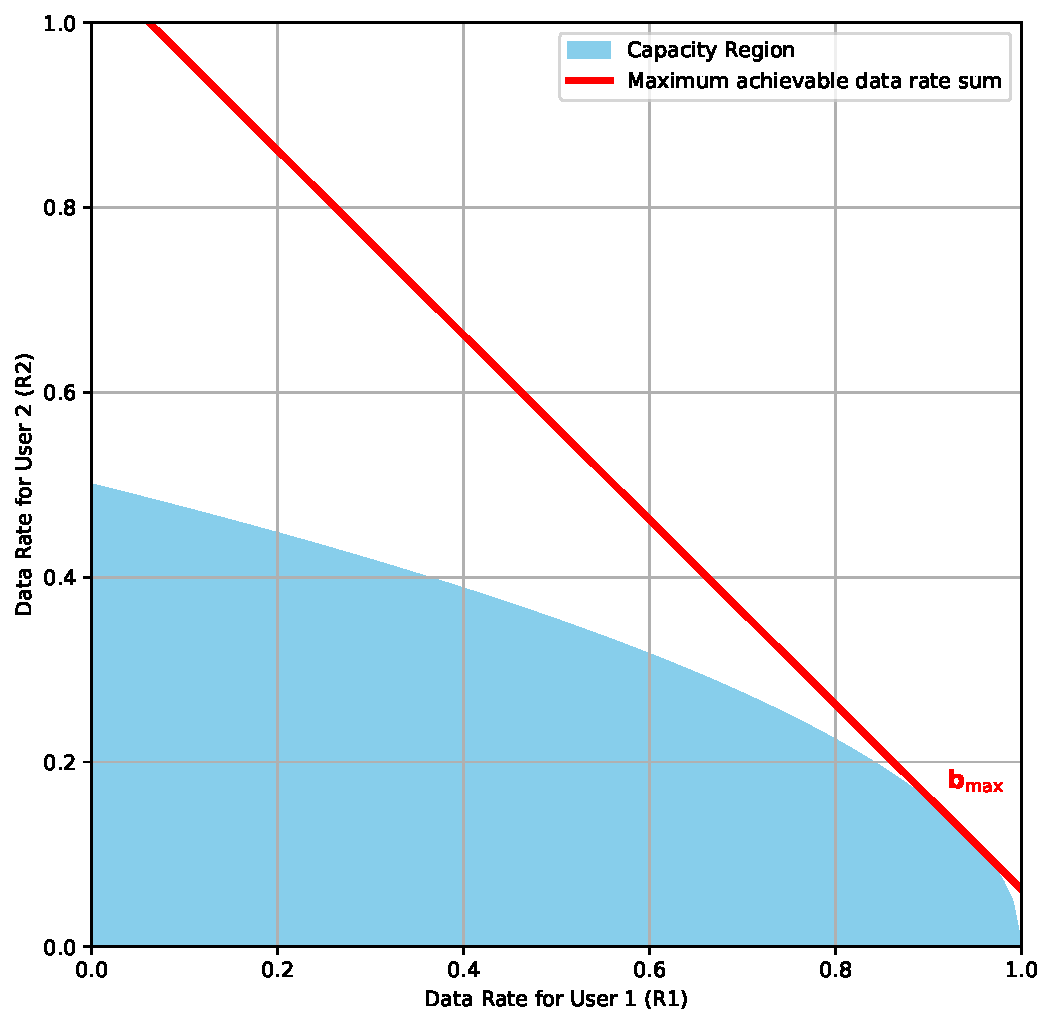
\includegraphics[width=6cm]{figures/Capacity_Region.pdf}
%     \caption{Capacity Region for two Users}
%     \label{fig:capacity_region}
% \end{figure}

% Repeat problem explanation
% Copy formulation from slides for energy minimization problem: explain and break it down into simpler subproblem by defining b, for example
% Explain GDFE from Chapter 5
% Explain minPMAC logic, ellipsoid, provide code from book , explain the concept of time sharing or vertex sharing
The Generalized Decision-Feedback Equalizer (GDFE) resolves multiuser crosstalk issues. To achieve this, each user's data is detected based on all previously decoded users with each symbol \cite{book}, \cite{yu2004sum}. % By assuming that the channel is non-singular, and we are using ideal code {\color{red} (Gap = 0)}, 

This work compares the performance of non-linear (GDFE) receivers \cite{GDFE} and linear receivers\cite{chang1966synthesis}, both using basic OFDM.  The specific focus is energy consumption. Initially, the receiver analysis uses the Simultaneous Water-Filling (SWF) algorithm\cite{book} with the linear receiver.  This SWF optimizes the sum data rate for a given available energy. Subsequently, a receiver uses the GDFE, targeting the data rate determined by the SWF algorithm, to minimize energy. The objective is to demonstrate how the GDFE receiver can substantially reduce energy consumption in attaining the same SWF data rate values obtained. 
% {\color{red} why GDFE results in a better energy preservation?}

Notation includes: $U$ denotes the number of users. $\bar{N}$ represents the number of tones. $L_x$ and $L_y$ are the total number of users' antennas and the total number of antennas at the access point, respectively. $L_{x,u}$ is the number of antennas for the $u^{th}$ user. Moreover, the subscripts $u$ and $n$ represent user $u$ and $n^{th}$ tone, respectively. For instance, $H_u$ is user $u$'s channel matrix. 
% The duality between these two problems arises from their shared Lagrangian frameworks. Both problems involve a common Lagrangian term in their expressions, which indicates a zero duality gap for their respective optimizations under certain conditions. The Lagrangian expressions for both problems differ in how the parameters $\theta$ and $w$ are interpreted (as either given constants or Lagrange multipliers) and in the terms related to incremental change constraints.
There are two weighted-sum optimization problems: Energy Sum Minimization (\ref{Esum}) and Data Rate Sum Maximization (\ref{Rsum}).
\subsection{Energy Sum Minimization} \label{Esum}
The weighted Energy Sum Minimization is formulated as follows:
\begin{equation}
\begin{aligned}
\min_{\left\{R_{\boldsymbol{xx}}{(u)} \right\}} \quad & \sum_{u=1}^U w_u \cdot \operatorname{trace} \underbrace{\{R_{ \boldsymbol{x} \boldsymbol{x}}{(u)}\}}_{\mathcal{E}_u}\\
\textrm{s.t.} \quad & \mathbf{b} \succeq \left[b_{1, \min }, b_{2, \min }, \ldots, b_{U, \min }\right]^*\\
  &\mathcal{E}\geq0    \\
\end{aligned}
\end{equation}
Where $R_{\boldsymbol{xx}}(u)$ and $b_{u,\operatorname{min}}$ are the autocorrelation matrix and user $u$'s minimum data rate, respectively. Also, the vector $w \in \mathbb{R}_{0+}^U$ represents non-negative weights for each user's energy.
The corresponding Lagrangian function is:
% \begin{equation}
% \begin{aligned}
% \mathcal{L}\left(R_{\boldsymbol{x} \boldsymbol{x}}(n), \boldsymbol{b}, \boldsymbol{w}, \boldsymbol{\theta}\right)=\sum_{u=1}^U(&w_u \cdot\left[\sum_{n=0}^{\bar{N}} \operatorname{trace}\left\{R_{\boldsymbol{x} \boldsymbol{x}}(u, n)\right\}\right]+\\
% &\theta_u \cdot\left\{\left[\sum_{n=0}^{\bar{N}-1} b_{u, n}\right]-b_u\right\})
% \end{aligned}
% \end{equation}
\begin{equation}
\begin{aligned}
\mathcal{L}_{\min E}\left(R_{\boldsymbol{x} \boldsymbol{x}}, \boldsymbol{b}, \boldsymbol{w}, \boldsymbol{\theta}\right)=\max _{\boldsymbol{\theta}} \min _{R_{\boldsymbol{x} \boldsymbol{x}}} &\sum_{u=1}^U  w_u \cdot \operatorname{trace}\left\{R_{\boldsymbol{x} \boldsymbol{x}}(u)\right\}\\ &+ \theta_u \cdot b_u-\theta_u \cdot b_{\min , u}
\end{aligned}
\end{equation}
\subsection{Data Rate Sum Maximization} \label{Rsum}
The weighted Data Rate Sum Maximization problem can be formulated as follows:
\begin{equation}
\begin{aligned}
\max _{\left\{R_{\boldsymbol{x} \boldsymbol{x}}{(u)}\right\}} \quad &\sum_{u=1}^U \theta_u \cdot b_u \\
\textrm{s.t.} \quad &\mathcal{E}_{\boldsymbol{x}} \preceq\left[\mathcal{E}_{1,\max}, \mathcal{E}_{2,\text{max}},\ldots,\mathcal{E}_{U,\text{max}}\right]^*\\
& \mathbf{b} \succeq 0
\end{aligned}
\end{equation}
Similar to the previous part, we can expand the Lagrangian function:
\begin{equation}
\begin{aligned}
\mathcal{L}_{\max R}\left(R_{\boldsymbol{x} \boldsymbol{x}}, \boldsymbol{b}, \boldsymbol{w}, \boldsymbol{\theta}\right)=\min _{\boldsymbol{w}} \max _{R_{\boldsymbol{x} \boldsymbol{x}}} &\sum_{u=1}^U w_u \cdot \operatorname{trace}\left\{R_{\boldsymbol{x} \boldsymbol{x}}(u)\right\}\\ &+\:\theta_u \cdot b_u-w_u \cdot \mathcal{E}_{\max , u}
\end{aligned}
\end{equation} 

The common term $w_u \cdot \operatorname{trace}\left\{R_{\boldsymbol{x} \boldsymbol{x}}(u)\right\} + \theta_u \cdot b_u$ in both optimization problems implies their duality. Therefore, a primal-dual approach solves the optimization problem.This locates the optimal autocorrelation matrix $R_{\boldsymbol{xx}}$, while fulfilling both the data rate and energy constraints. 
% Both problems involve a common Lagrangian term in their expressions, which indicates a zero duality gap for their respective optimizations under certain conditions. The Lagrangian expressions for both problems differ in how the parameters $\theta$ and $w$ are interpreted (as either given constants or Lagrange multipliers) and in the terms related to incremental change constraints.


% As we can see, there is a common term in both optimization problems, and our algorithm tries to optimize these two problems simultaneously. Specifically, the algorithm locates the optimal $R_{\boldsymbol{xx}}$, while fulfilling both the data rate and energy constraints. 
It can be proven that the aforementioned optimization problems can be solved for each tone separately. In other words, an independent GDFE is assigned to each tone, and the total energy can be calculated by summing up all tones\cite{book}. The corresponding energy minimization problem for each tone is as follows:
\begin{equation} \label{tonalE}
    \begin{aligned}
        \min_{\left\{R_{\boldsymbol{x} \boldsymbol{x}}{(u, n)}\right\}} \quad &\sum_{u=1}^U \sum_{n=0}^{\bar{N}} w_u \cdot \operatorname{trace}\left\{R_{\boldsymbol{x} \boldsymbol{x}}(u, n)\right\} \\
        \textrm{s.t.} \quad &\mathbf{b}=\sum_{n=0}^{\bar{N}}\left[b_{1, n}, b_{2, n}, \ldots ,b_{U, n}\right]^* \succeq \boldsymbol{b}_{\min } \succeq \mathbf{0}
    \end{aligned}
\end{equation}
Where $R_{\boldsymbol{xx}}(u,n)\in\mathbb{R}^{L_{x,u}\times L_{x,u}}$ is the autocorrelation matrix of $\boldsymbol{x}$ for user $u$ on the $n^{th}$ tone. 

Similarly, the data rate maximization problem per each tone is:
\begin{equation}
\begin{aligned}
\max_{\left\{R_{\boldsymbol{x} \boldsymbol{x}}{(u, n)}\right\}} \quad &\sum_{u=1}^U \theta_u \cdot\left\{\sum_{n=0}^{\bar{N}} b_{u, n}\right\} \\
\textrm{s.t.} \quad &\mathcal{E}=\sum_{n=0}^{\bar{N}}\left[\mathcal{E}_{1, n}, \mathcal{E}_{2, n}, \ldots, \mathcal{E}_{U, n}\right]^* \preceq \boldsymbol{\mathcal{E}}_{\max } \;\;.
\end{aligned}
\end{equation}
Equation \ref{tonalE} 's Lagrangian function is:
\begin{equation} \label{minmaxE}
\begin{aligned}
\mathcal{L}_{\min E}\left(R_{\boldsymbol{x} \boldsymbol{x}}, \boldsymbol{b}, \boldsymbol{w}, \boldsymbol{\theta}\right)&=\left(\sum_{u=1}^U \theta_u \cdot b_u\right)
+ \\
& \hspace{-1.5cm} \sum_{n=0}^{\bar{N}-1}\{\underbrace{\sum_{u=1}^U\left[w_u \cdot \operatorname{trace}\left\{R_{\boldsymbol{x} \boldsymbol{x}}(u, n)\right\}-\theta_u \cdot b_{u, n}\right]}_{\mathcal{L}_n\left(R_{\boldsymbol{x} \boldsymbol{x}}(n), \boldsymbol{b}_n, \boldsymbol{w}, \boldsymbol{\theta}\right)}\}
\end{aligned}
\end{equation}
Where $R_{\boldsymbol{x} \boldsymbol{x}}(n)=\operatorname{blkdiag}\left\{R_{\boldsymbol{x} \boldsymbol{x}}(U, n), \ldots, R_{\boldsymbol{x} \boldsymbol{x}}(1, n)\right\}$, and the operator $\operatorname{blkdiag}$ aligns matrices along the diagonal of another matrix. The term $\mathcal{L}_n\left(R_{\boldsymbol{x} \boldsymbol{x}}(n), \boldsymbol{b}_n, \boldsymbol{w}, \boldsymbol{\theta}\right)$ is called the Tonal Lagrangian term. Since $\mathcal{L}_n$ does not depend on $b_u$, minimizing the tonal lagrangian term is synonymous with optimizing: 
\begin{equation}
\mathcal{L}_{\min E}(\boldsymbol{\theta}, n) \triangleq \min _{\left\{R_{\boldsymbol{xx}}(u, n), b_{u, n}\right\}} \mathcal{L}\left(R_{\boldsymbol{xx}}(n), \boldsymbol{b}_n, \boldsymbol{w}, \boldsymbol{\theta}\right)    
\end{equation}
Therefore, the min-max problem \ref{minmaxE} reduces to :
\begin{equation} \label{final}
\mathcal{L}_{\min E}^*=\max _{\boldsymbol{\theta}}\{\left[\sum_{n=0}^{\bar{N}-1} \mathcal{L}_{\min E}(\boldsymbol{\theta}, n)\right]+\hspace{-0.5cm}\underbrace{\sum_{u=1}^U \theta_u \cdot b_u}_{\text {independent of } R_{\boldsymbol{xx}}(u, n), n}\hspace{-0.5cm}\}
\end{equation}

Moreover, the data rates must lie in the system's capacity region. The capacity region, denoted as $\mathcal{C}(b)$, refers to the set of all possible rate vectors $b$ for users with independent messages, where each message employs a code that achieves the single-user capacity. This code is used for all systems and differences in their performance therefore solely derives from the GDFE improvement over the linear receiver.  This set characterizes the rates at which all users can be reliably decoded with a negligible average error probability by a Maximum A Posteriori (MAP) detector or equivalently, a Maximum Likelihood (ML) detector with equally likely messages for all independent users. The capacity region is essentially the combination of rates at which the system can operate such that all users' messages are delivered correctly. %Figure \ref{fig:capacity_region} depicts the capacity region for two users. 
The capacity region follows from the Shannon capacity formula as \cite{shannon}: 
\begin{equation}
0 \leq b_n %\sum_{\boldsymbol{u} \subseteq \boldsymbol{U}} b_{u, n}
\leq \log _2\left|\left(\sum_{u=1}^U \widetilde{H}_{u, n} \cdot R_{\boldsymbol{x} \boldsymbol{x}}(u, n) \cdot \widetilde{H}_{u, n}^*\right)+I\right|
\end{equation}

$\tilde{H}_{u, n}=R_{N N}^{-1 / 2}(n) \cdot H_{u, n}$ is the equivalent-white-noise channel per each tone.
% A multiple-input-multiple-output (MIMO) system with additive white Gaussian noise (AWGN) can be described as
% \begin{equation}
% \boldsymbol{y}=H \cdot \boldsymbol{x}+\boldsymbol{n}
% \end{equation}

% Where $H \in \mathbb{R}^{L_y \times L_x}$ is the channel matrix, and $x$, $y$ are the transmitted and received signals respectively. 
A semi-definite programming (SDP) method solves the inner part of the optimization problem \ref{final} ($\mathcal{L}_{\min E}(\boldsymbol{\theta}, n)$), while an Ellipsoid method \cite{yudin1976constrained} 
% {\color{red} Correct the citation part} optimizes the outer part. 

If the channel matrix $H_{u,n}$ is non-singular with the ideal common codes mentioned ($\Gamma = 0 \textrm{dB}$), the ellipsoid method finds a unique optimal solution. In other words, the system assigns different dimensions, such as time and frequency, to each user separately. However, if the channel is singular, the Hessian matrix computed at each ellipsoid-method iteration degradeds, and the optimization problem does not have a unique solution. In this case, the algorithm allows more than one user to use some specific dimensions at the same time, which is known as “time-sharing”. When the users “time-share” with one another, the algorithm only finds the weighted sum.  A separate time-sharing step then applies to ensure all users meet their target data rate.  

% If the optimal point of energy lies inside the capacity-energy region, the Ellipsoid algorithm can find this point successfully. However, as we get closer to the boundary of the capacity region, the Hessian matrix constructed in the Ellipsoid algorithm will become singular (the minimum eigenvalue of the Hessian matrix will get closer to zero). Under these conditions, the system is stressed, making it more challenging for the Ellipsoid method to converge.

% {\color{red}this paragraph or above} Our algorithm is capable of stressing the system as much as possible so that each user doesn't experience low data rate. However, this goal is within reach only by using time-sharing, which is synonymous with allowing users to use the same amount of resources at the same time.

This minPMAC algorithm appears as Algorithm 2.  Initially, the SWF algorithm provides first ellipsoid parameters. Then, minPMAC alternates between two optimization problems until convergence. It prioritizes the users' decoding process based on $\theta$ at each iteration.

% \begin{table}[t]
%     \caption{Notation Explanation}
%     \centering
%     \begin{tabular}{|c|c|}
%     \hline
%        \textbf{Parameter}  &  \textbf{Explanation}\\ \hline
%        $U$ & Number of users\\ 
%        $N$ & Number of tones\\
%        $L_x$ & Total number of users' antennas\\
%        $L_y$ & Total number of antennas at the access point\\ 
%        $L_{x,u}$ & user $u^{th}$ number of  antennas \\  \hline
        
%     \end{tabular}
%     \label{tab:ranging-imu-params}
% \end{table}



\begin{algorithm}[t]
	\caption{SWF} 
    \State \textbf{Inputs:} $H, L_x, R_{nn}$
		\For {$u=1,2,\ldots,U$}
            \State $R_{\text {noise}}(u) \triangleq \sum_{i \neq u} H_i \cdot R_{\boldsymbol{x} \boldsymbol{x}}(i) \cdot H_i^*+R_{\boldsymbol{nn}}$
            \vspace{0.1cm}\State $R_{\text {noise }}^{-1 / 2}(u) \cdot H_u=F_u \cdot \Lambda_u \cdot M_u^*$
            \vspace{0.1cm}\For{$\ell = 1,2,\ldots, L_x$}
                \State $\mathcal{E}_{u,\ell} = \operatorname{max} \left\{0, {\frac{1}{L_x}}\left(\mathcal{E}_u - \sum_{k=1}^{L_x}\frac{1}{\lambda_{u,k}^2}\right) - \frac{1}{\lambda_{u,\ell}^2}\right\}$
            \vspace{0.1cm}
            \EndFor
		\EndFor
\State \textbf{return} $\mathcal{E}_u$
\end{algorithm}







% \vspace{30 pt}

\begin{algorithm}[t]
	\caption{minPMAC} 
	% \begin{algorithmic}[1]
    \State \textbf{Inputs:} $H$, $L_{xu}$, $b_u$, $w$ 
    \vspace{0.1cm}
    \State \textbf{Initialize:} $A$, $\theta$ using SWF
    % \vspace{0.1cm}
    % \State $Idx_{END} = \operatorname{cumsum}(L_{xu})$
    % \vspace{0.1cm}
    % \State $Idx_{START} = [1, Idx_{END}(1:end-1)+1]$ 
    % \vspace{0.1cm}
    % \State $D \in \mathbb{R}^{U\times U}, \quad D_{i,i} = 1, D_{i,i+1} = -1 \quad \forall 1\leq i \leq U-1$
    % \vspace{0.1cm}
    \While {the sum rate doesn't converge}
    \vspace{0.1cm}
    \State $\pi \triangleq$ Indices of sorted $\theta$ in descending order
    \vspace{0.1cm}
       \For {$n = 1,2, \ldots,\bar{N}$}
        \vspace{0.1cm}
            \For{$u = 1,2,\ldots,U$}
                \vspace{0.1cm}
                \State \hspace{-0.3cm} $\footnotesize \mathcal{E}_{u,n} = \operatorname{trace}\left(R_{\boldsymbol{x} \boldsymbol{x}}\left(\pi^{-1}(u), n\right)\right)$
                \vspace{0.1cm}
                \State \hspace{-0.3cm} $\footnotesize \mathcal{R}_{u,n} \triangleq  \log _2\left|\sum_{i=u}^U \tilde{H}_{\pi^{-1}(i), n} \cdot R_{\boldsymbol{x} \boldsymbol{x}}\left(\pi^{-1}(i), n\right) \cdot \tilde{H}_{\pi^{-1}(i), n}^*+I\right|$
            \EndFor 
            \vspace{-0.7cm}
            \State \begin{equation*}
            \hspace{0.5cm} b_{u,n}^*=\underset{{R_{\boldsymbol{xx}}}}{\operatorname{argmin}} \quad \sum_{u=1}^U w_{u} \cdot \: \mathcal{E}_{u,n}- \left(\theta_{\pi^{-1}(u)}-\theta_{\pi^{-1}(u+1)}\right) \cdot \: \mathcal{R}_{u,n} \end{equation*}
            \vspace{-0.6cm}
            \State \begin{equation*}
                \hspace{-2cm} \textrm{s.t.} \quad R_{\boldsymbol{xx}}  \succeq \mathbf{0}
            \end{equation*}
    \EndFor 
    \vspace{0.1cm}
    \State $g = \sum_{n = 1}^{\bar{N}}  b_{u,n}^* - b_u$
    \vspace{0.1cm}
	\State $\tilde{g} = \frac{1}{\sqrt[]{g^TAg}}g$
    \vspace{0.1cm}
    \State $\theta = \theta - \frac{1}{U+1}\frac{Ag}{\sqrt[]{g^TAg}}$
    \vspace{0.1cm}
    \State $A = \frac{U^2}{U^2-1}(A - \frac{2}{U+1} A \tilde{g}\tilde{g}^T A)$
    % \vspace{0.1cm}
    % \State $\mathcal{S} = \left\{i \: | \: \theta_i < 0\right\}$
    % \vspace{0.1cm}
    % \While {$\mathcal{S} \neq \left\{\right\}$}
    %     \State $g = \mathbf{0}$
    %     \vspace{0.1cm}
    %     \State $g(\mathcal{S}(1)) = 1$
    %     \vspace{0.1cm}
    % 	\State $\tilde{g} = \frac{1}{\sqrt[]{g^TAg}}g$
    %     \vspace{0.1cm}
    %     \State $\theta = \theta - \frac{1}{U+1}\frac{Ag}{\sqrt[]{g^TAg}}$
    %     \vspace{0.1cm}
    %     \State $A = \frac{U^2}{U^2-1}(A - \frac{2}{U+1} A \tilde{g}\tilde{g}^T A)$
    %     \vspace{0.1cm}
    %     \State $\mathcal{S} = \left\{i \: | \: \theta_i < 0\right\}$
    % \ENDWHILE
\ENDWHILE
\vspace{0.1cm}
\State \textbf{return} $b_{u,n}^*, \: \mathcal{E}_{u,n}$
\end{algorithm}


\section {Performance Evaluation}

\begin{table}[t]
    \caption{Experiment Parameters}
    \centering
    \resizebox{7.5cm}{!}{
    \begin{tabular}{|c|c|}
    \hline
      Parameter & Value \\
    \hline
      Number of users $N$ & \{2, 3\} \\
      Number of antennas per user $L_{xu}$ & 1 \\
      Number of antennas at AP $L_y$ & \{2, 3, 4\} \\
      User to AP distance range $[d_{min}, d_{max}]$ & [1m, 10m]\\
      Channel bandwidth $W$ & 100 MHz \\
      Number of channel delay taps $n_{delay}$ & \{9, 18\} \\
      FFT length ${fft}_{length}$ & \{16, 32, 64, 128, 256\} \\
      SNR & [-10, 50] dB \\
    \hline
    \end{tabular}}
    \label{tab:experiment-parameters}
\end{table} 
\begin{figure}
    \centering
    \begin{subfigure}[b]{8cm}
    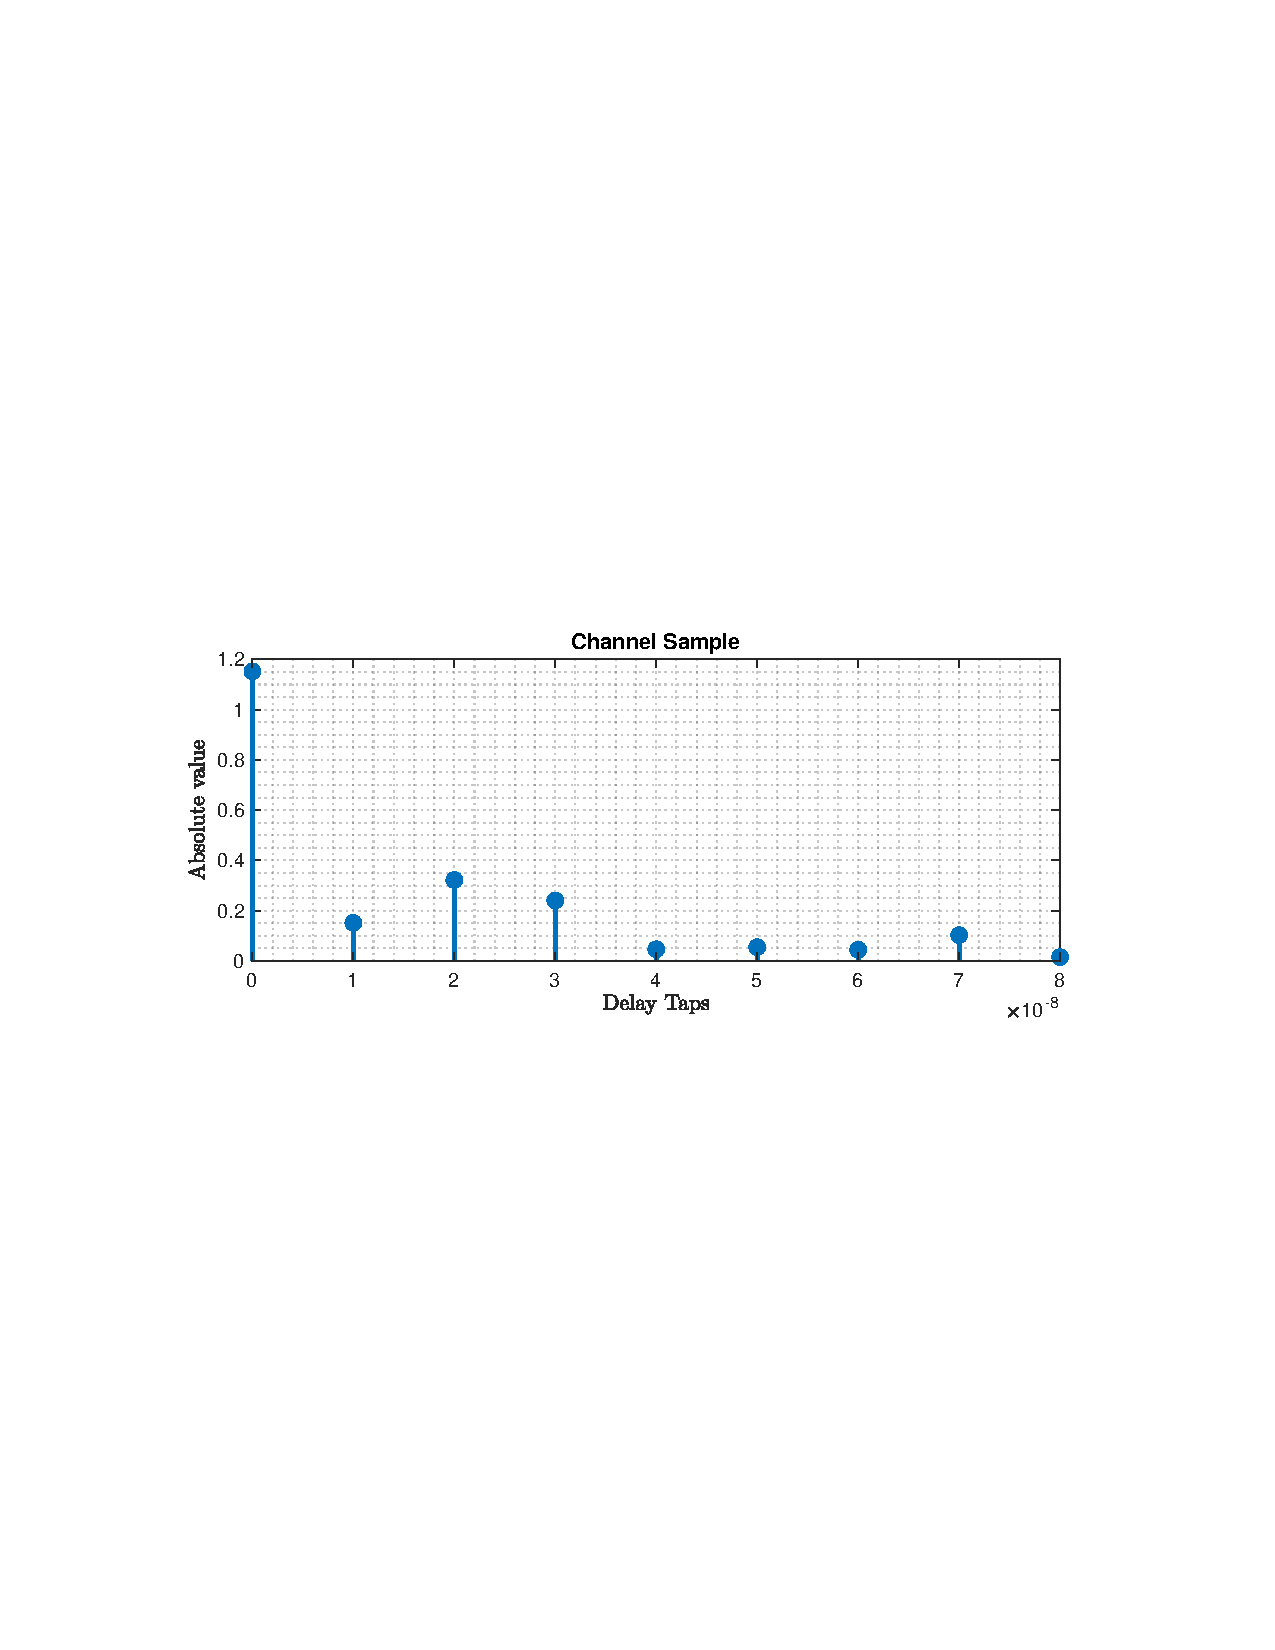
\includegraphics[trim={3cm 10.7cm 3cm 10cm},clip, width=8cm]{figures/TimeSample_2.pdf}
    \end{subfigure}
    \begin{subfigure}[b]{8 cm}
    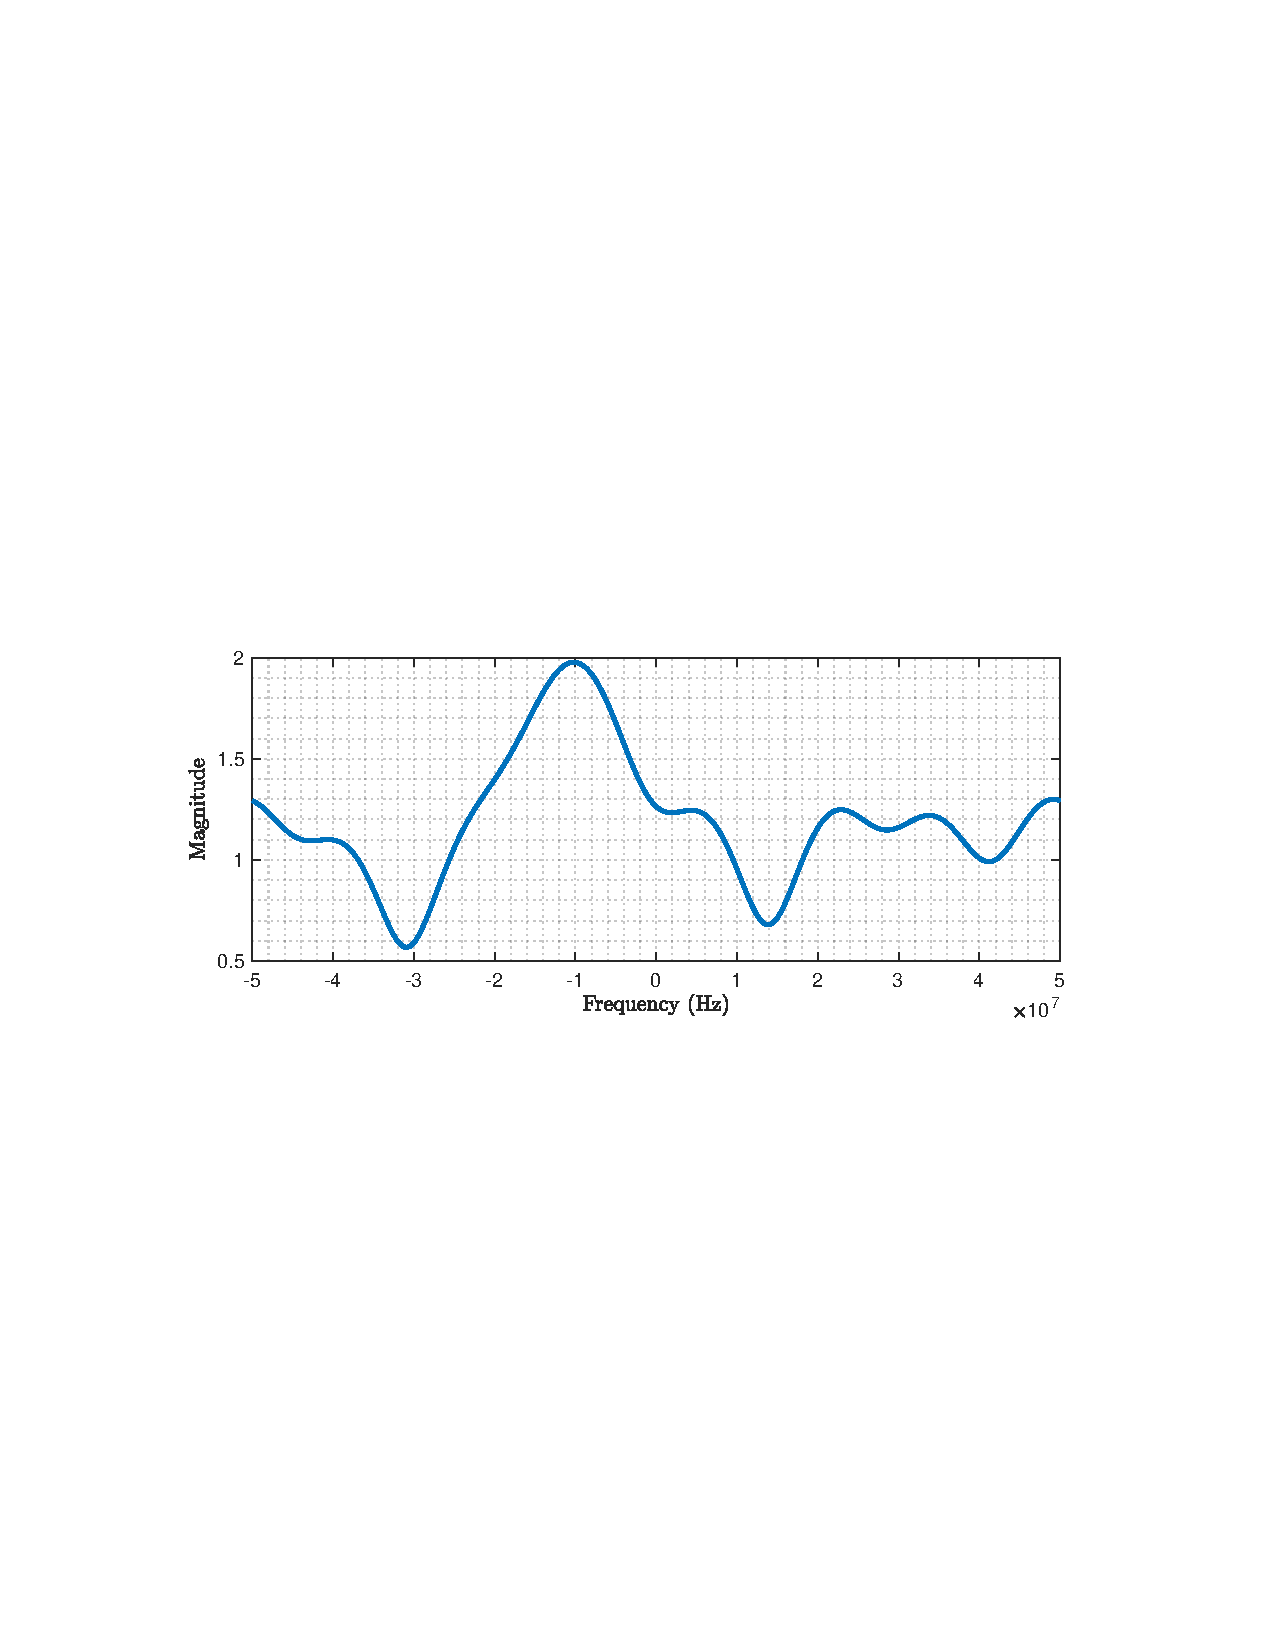
\includegraphics[trim={3cm 10.7cm 3cm 10cm},clip, width=8cm]{figures/FreqSample_2.pdf}   
    \end{subfigure}
    \caption{Channel B Samples}
    \label{fig:channel-samples}
\end{figure}

\begin{table}[t]
    \caption{Parameters for 2 Experiment Scenarios}
    \centering
    \resizebox{8.5cm}{!}{
    \begin{tabular}{|c|c|c|}
    \hline 
    \textbf{Parameter}& \textbf{Case 1}& \textbf{Case 2}\\
    \hline 
    \textbf{Antennas/user}& 1 & 1 \\
    \textbf{AP Antennas}& 2 & 2\\
    \textbf{Users}& 2 & 3 \\
    \textbf{Distance from AP (m)}& \{3, 3\} & \{3, 3, 3\} \\
    \hline
    \textbf{Data Rates (OFDM) (Mbps)}& \{239, 481\} & \{136, 236, 266\} \\
    \textbf{Data Rates (Proposed) (Mbps)}& \{239, 481\} & \{470, 470, 470\}\\
    \hline
    \textbf{Energy (OFDM)}& \{1, 1\} & \{1, 1, 1\} \\
    \textbf{Energy (Proposed)}& \{0.1168, 0.2870\} & \{0.3437, 0.9621, 0.9308\} \\
    \hline 
    \end{tabular}}
    \label{tab:scearios-single}
\end{table}


% \begin{table}[t]
% \caption{Energy Consumption versus Number of AP Antennas for Single Antenna Per User, $U = 3$, $L_{xu} = 1$, $\textrm{distance from AP} = \{3m,3m,3m\}$}
% \centering
% \begin{tabular}{|c|c|c|}
% \hline
% \multirow{2}{*}{\textbf{AP Antennas}} & \multicolumn{2}{c|}{\textbf{Average Energy}} \\ \cline{2-3} 
%                      & \textbf{ OFDM} & \textbf{GDFE}  \\ \hline
% 1                    & 1                             & 0.5383         \\ \hline
% 2                    & 1                             & 0.1246         \\ \hline
% 3                    & 1                             & 0.0898         \\ \hline
% 4                    & 1                             & 0.1401         \\ \hline
% \end{tabular}
% \label{tab:my_label}
% \end{table}



\begin{table}[t]
\caption{Energy Consumption versus Number of AP Antennas for Single Antenna Per User, $R = 201.702 \textrm{ Mbps}$, $U = 3$, $L_{xu} = 1$, $\textrm{distance from AP} = \{3m,3m,3m\}$}
\centering
\resizebox{9cm}{!}{
\begin{tabular}{|c|c|c|c|c|}
\hline
\multirow{2}{*}{\begin{tabular}[c]{@{}c@{}}\textbf{AP} \\ \textbf{Antennas}\end{tabular}} & \multicolumn{2}{c|}{\textbf{OFDM}} & \multicolumn{2}{c|}{\textbf{Proposed Algorithm}} \\ \cline{2-5} 
                     & \textbf{Energy}& \textbf{$\textrm{Energy}_{\textrm{avg}}$}& \textbf{Energy}& \textbf{$\textrm{Energy}_{\textrm{avg}}$}\\ \hline
1                    & [1,  1,  1] & 1& [0.5721,    0.5417,    1.1325]& 0.7488\\ \hline
2                    & [0.9, 0.9,  0.9] & 0.9& [0.1354,    0.0422,    0.1552]& 0.1109\\ \hline
3                    & [0.75, 0.75, 0.75] & 0.75& [0.0294,    0.0750,    0.0893]& 0.0646\\ \hline
4                    & [0.3, 0.3, 0.3] & 0.3& [0.0214,    0.0508,    0.0556]& 0.0426\\ \hline
\end{tabular}}
\label{tab:energy-compare}
\end{table}
\begin{table}[t]
\caption{Energy Consumption versus Number of AP Antennas for Single Antenna Per User, Fixed energy for OFDM, $U = 3$, $L_{xu} = 1$, $\textrm{distance from AP} = \{3m,3m,3m\}$}
\centering
\resizebox{9cm}{!}{
\begin{tabular}{|c|c|c|c|c|}
\hline
\multirow{2}{*}{\begin{tabular}[c]{@{}c@{}}\textbf{AP} \\ \textbf{Antennas}\end{tabular}} & \multicolumn{2}{c|}{\textbf{OFDM}} & \multicolumn{2}{c|}{\textbf{Proposed Algorithm}} \\ \cline{2-5} 
                     & \textbf{Energy}& \textbf{Data Rates}& \textbf{Energy}& \textbf{Data Rates}\\ \hline
1                    & [1,  1,  1] & [204,  174,  175]& [1.1534,    0.5194,    0.7641]& [204,  174,  175]\\ \hline
2                    & [1,  1,  1] & [224,   87,  210]& [0.0259,    0.1662,    0.1737]& [87,  164,  270]\\ \hline
3                    & [1,  1,  1] & [233,  117,  200]& [0.0233,    0.1171,    0.1223]& [18,   210,  322]\\ \hline
4                    & [1,  1,  1] & [290,  180,  252]& [0.1818,    0.1738,    0.0938]& [408,  202,  112]\\ \hline
\end{tabular}}
\label{tab:energy-compare2}
\end{table}
\begin{figure}[t]
    \centering
    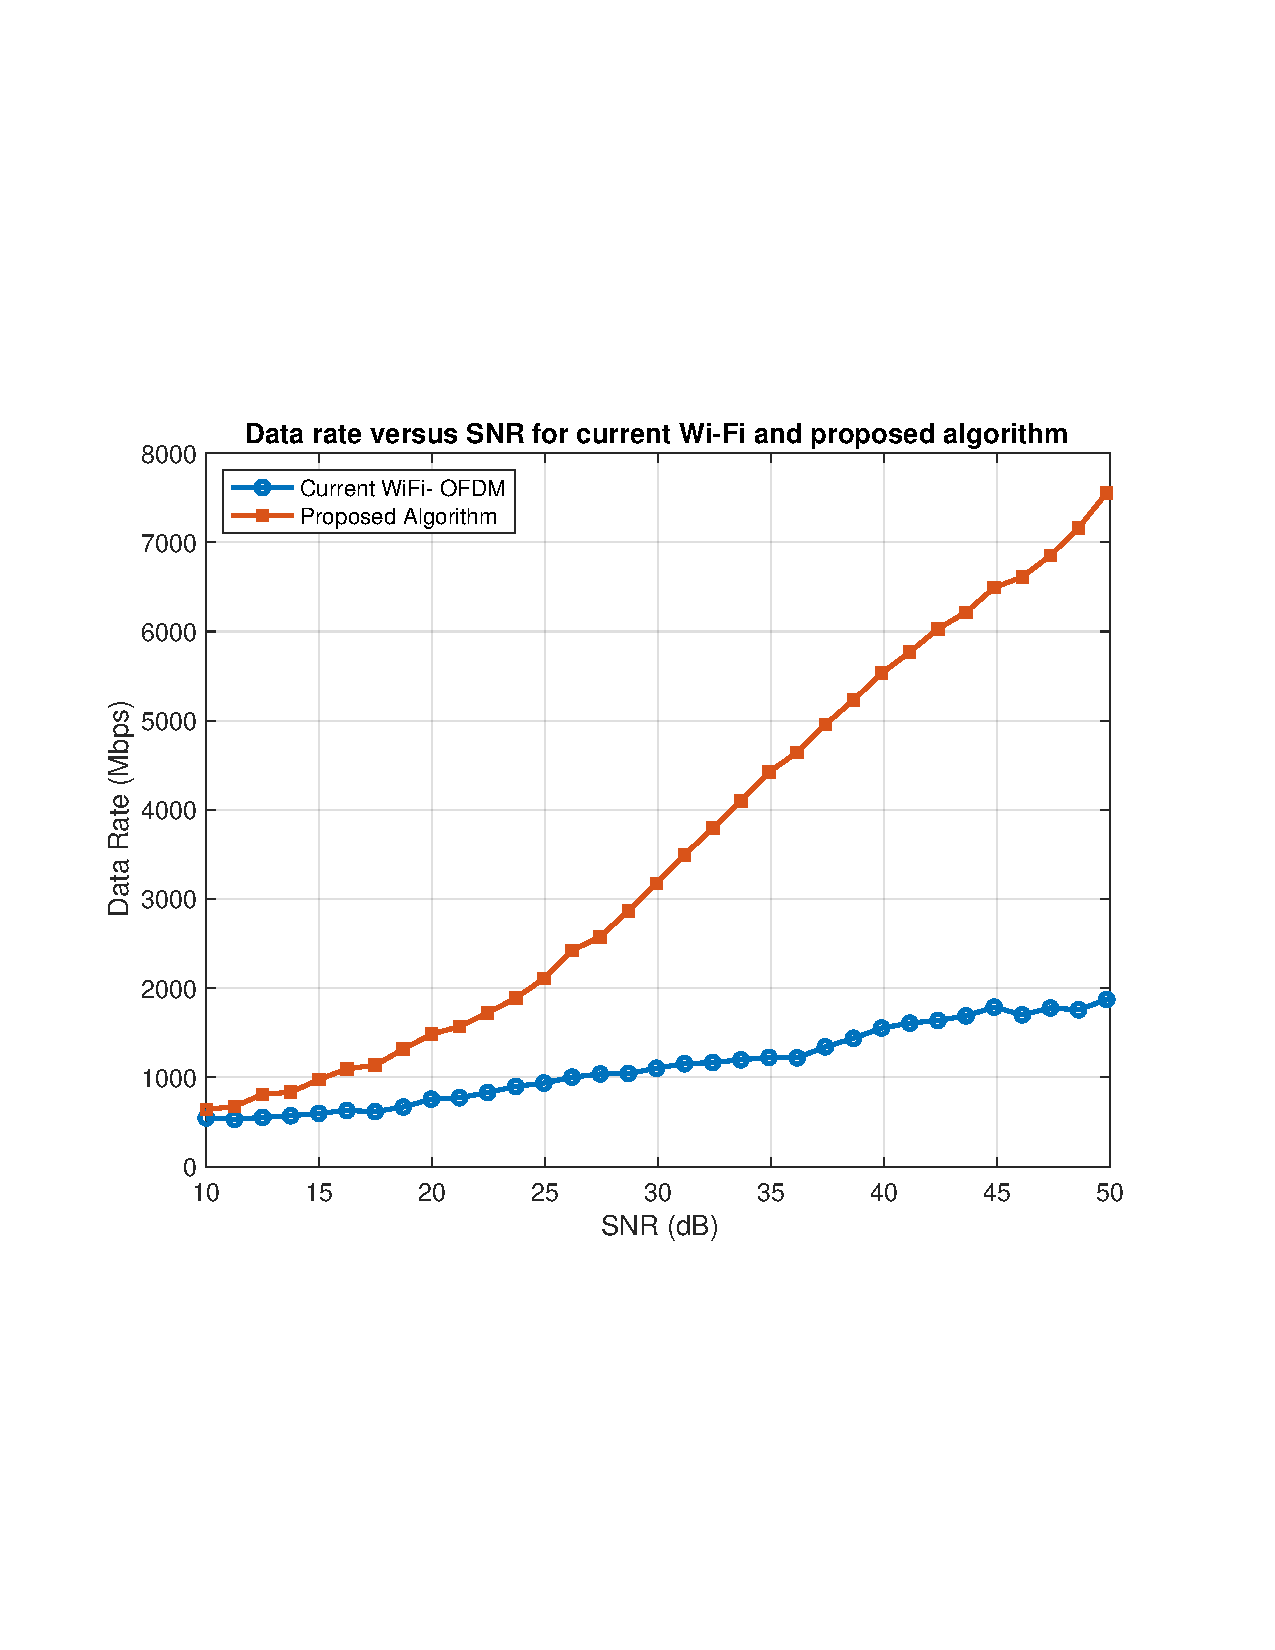
\includegraphics[trim = {30, 180, 10, 200}, clip, height = 6.3cm]{figures/data_rate_versus_SNR.pdf}
    \caption{Sum Rate versus SNR for Single Antenna Per User: Current Wi-Fi OFDM and Proposed Algorithm}
    \label{fig:data-rate-snr-single}
\end{figure}
\begin{figure}
    \centering
    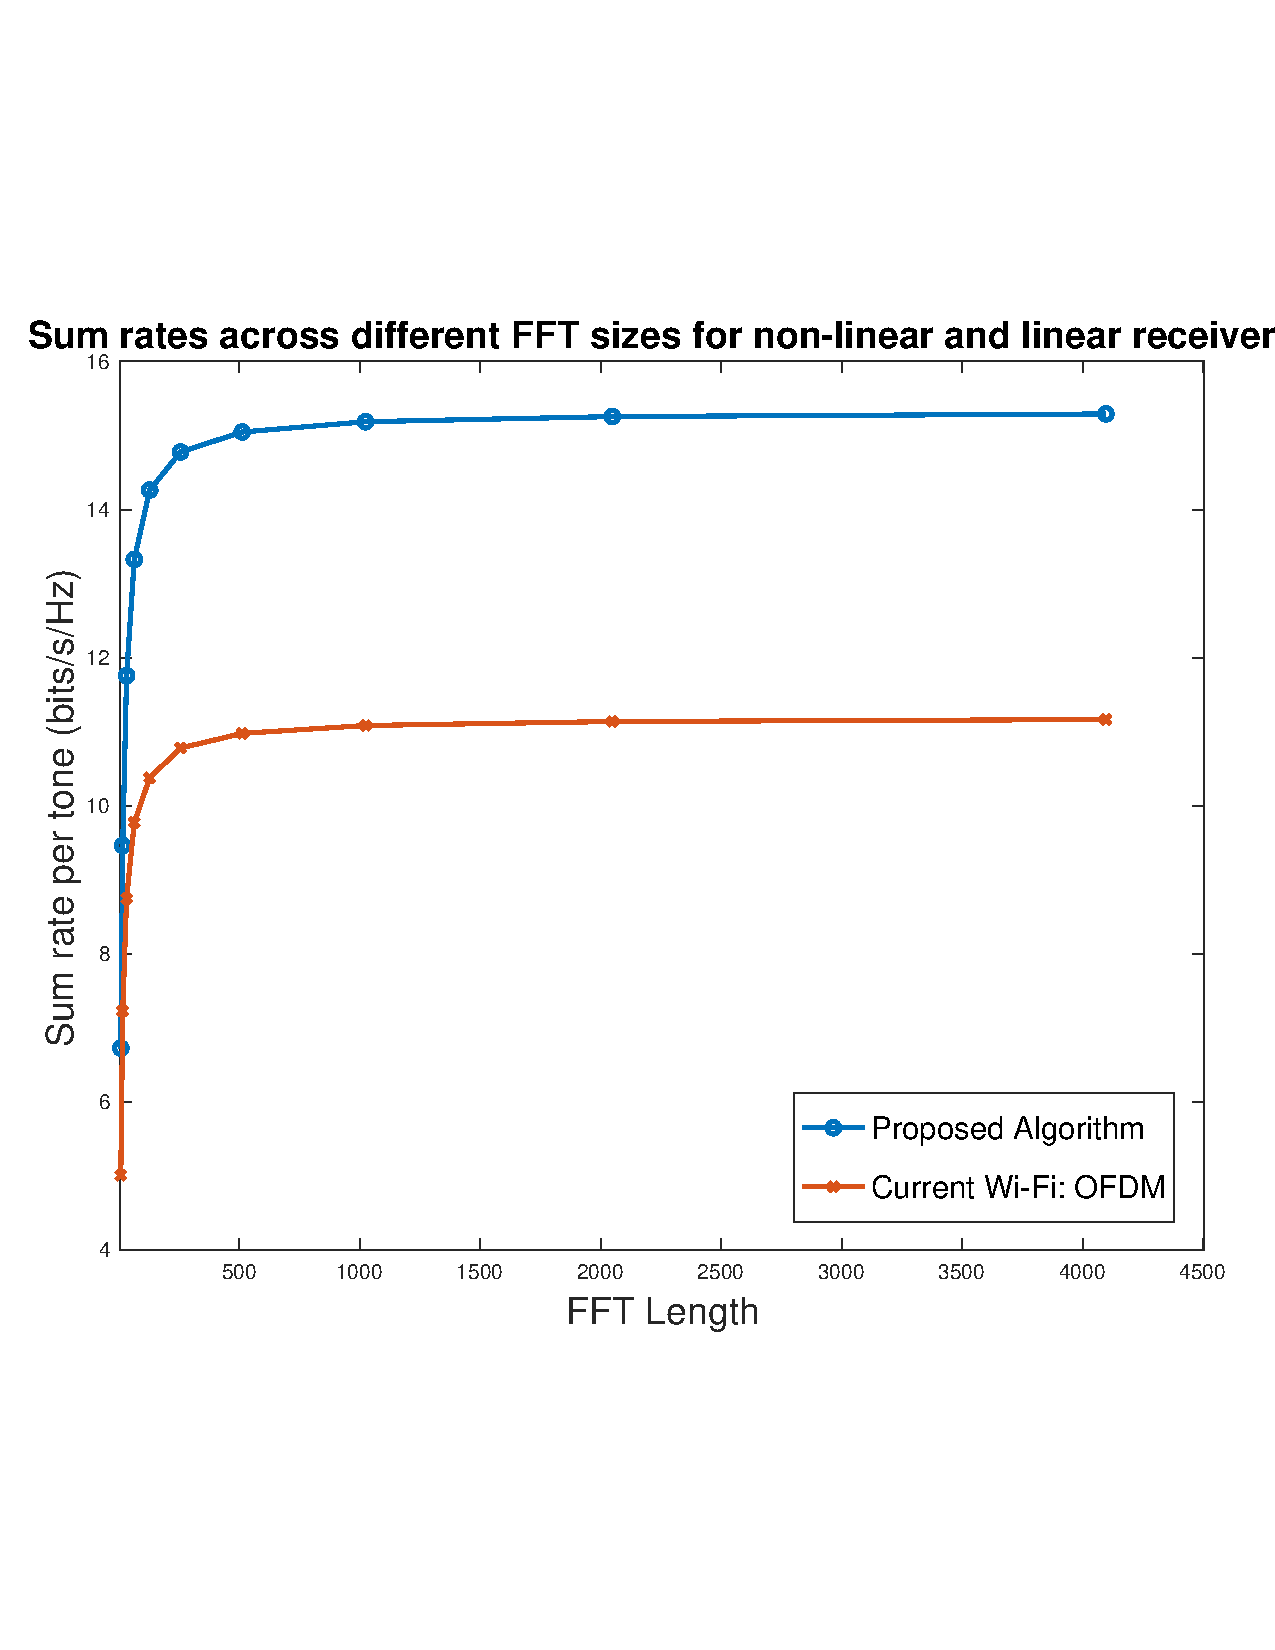
\includegraphics[trim = {0, 150, 0, 130}, clip, height = 7cm]{figures/3UsersEqualDistance3mSumRatePerTone.pdf}
    \caption{Sum rate versus FFT length for equidistant users with single antenna per user}
    \label{fig:data-rate-fft-single}
\end{figure}
\begin{figure}
    \centering
    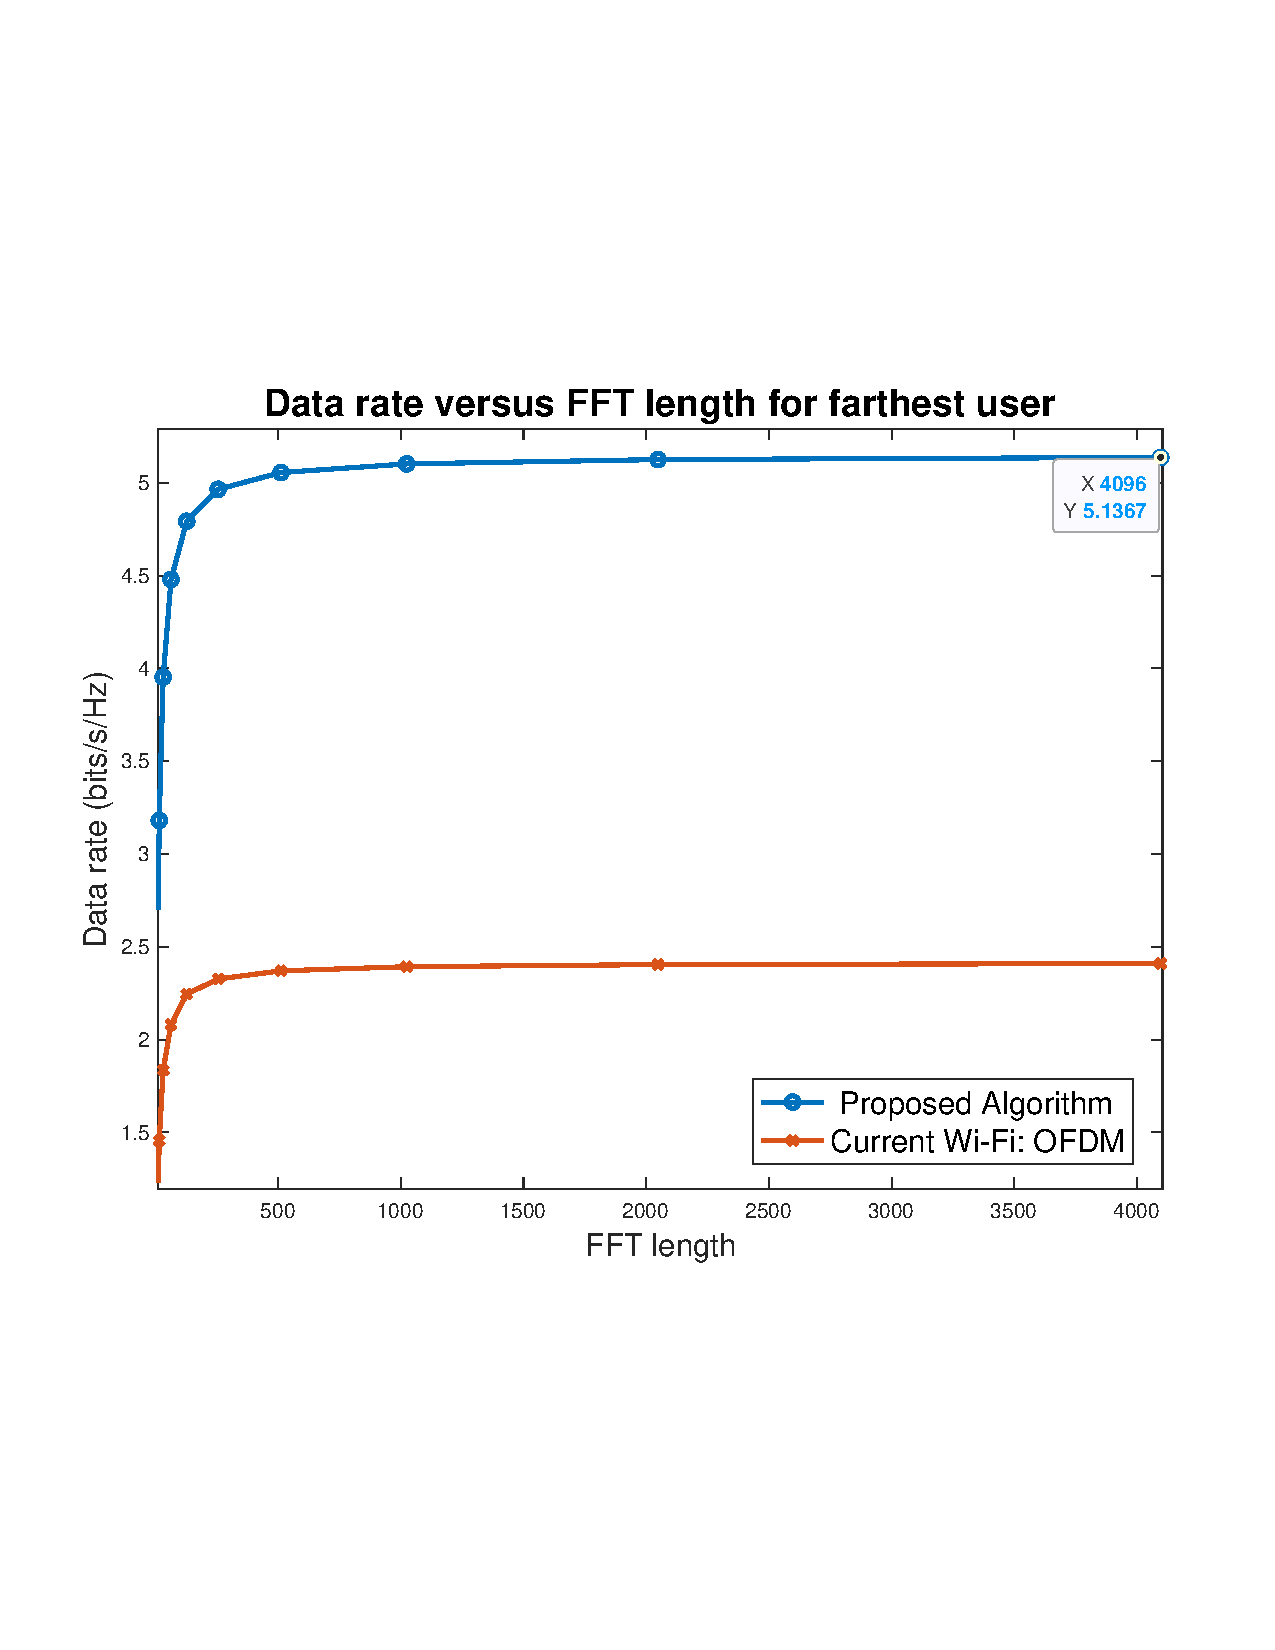
\includegraphics[trim = {20, 180, 0, 180}, clip, height = 7cm]{figures/3Users3_5_8mFarthestUserRatePerTone.pdf}
    \caption{Data rate versus FFT length for the farthest user with user distances from AP = \{3m, 5m, 8m\}, and single antenna per user}
    \label{fig:data-rate-farthest-fft-single}
\end{figure}
% \begin{figure}
%     \centering
%     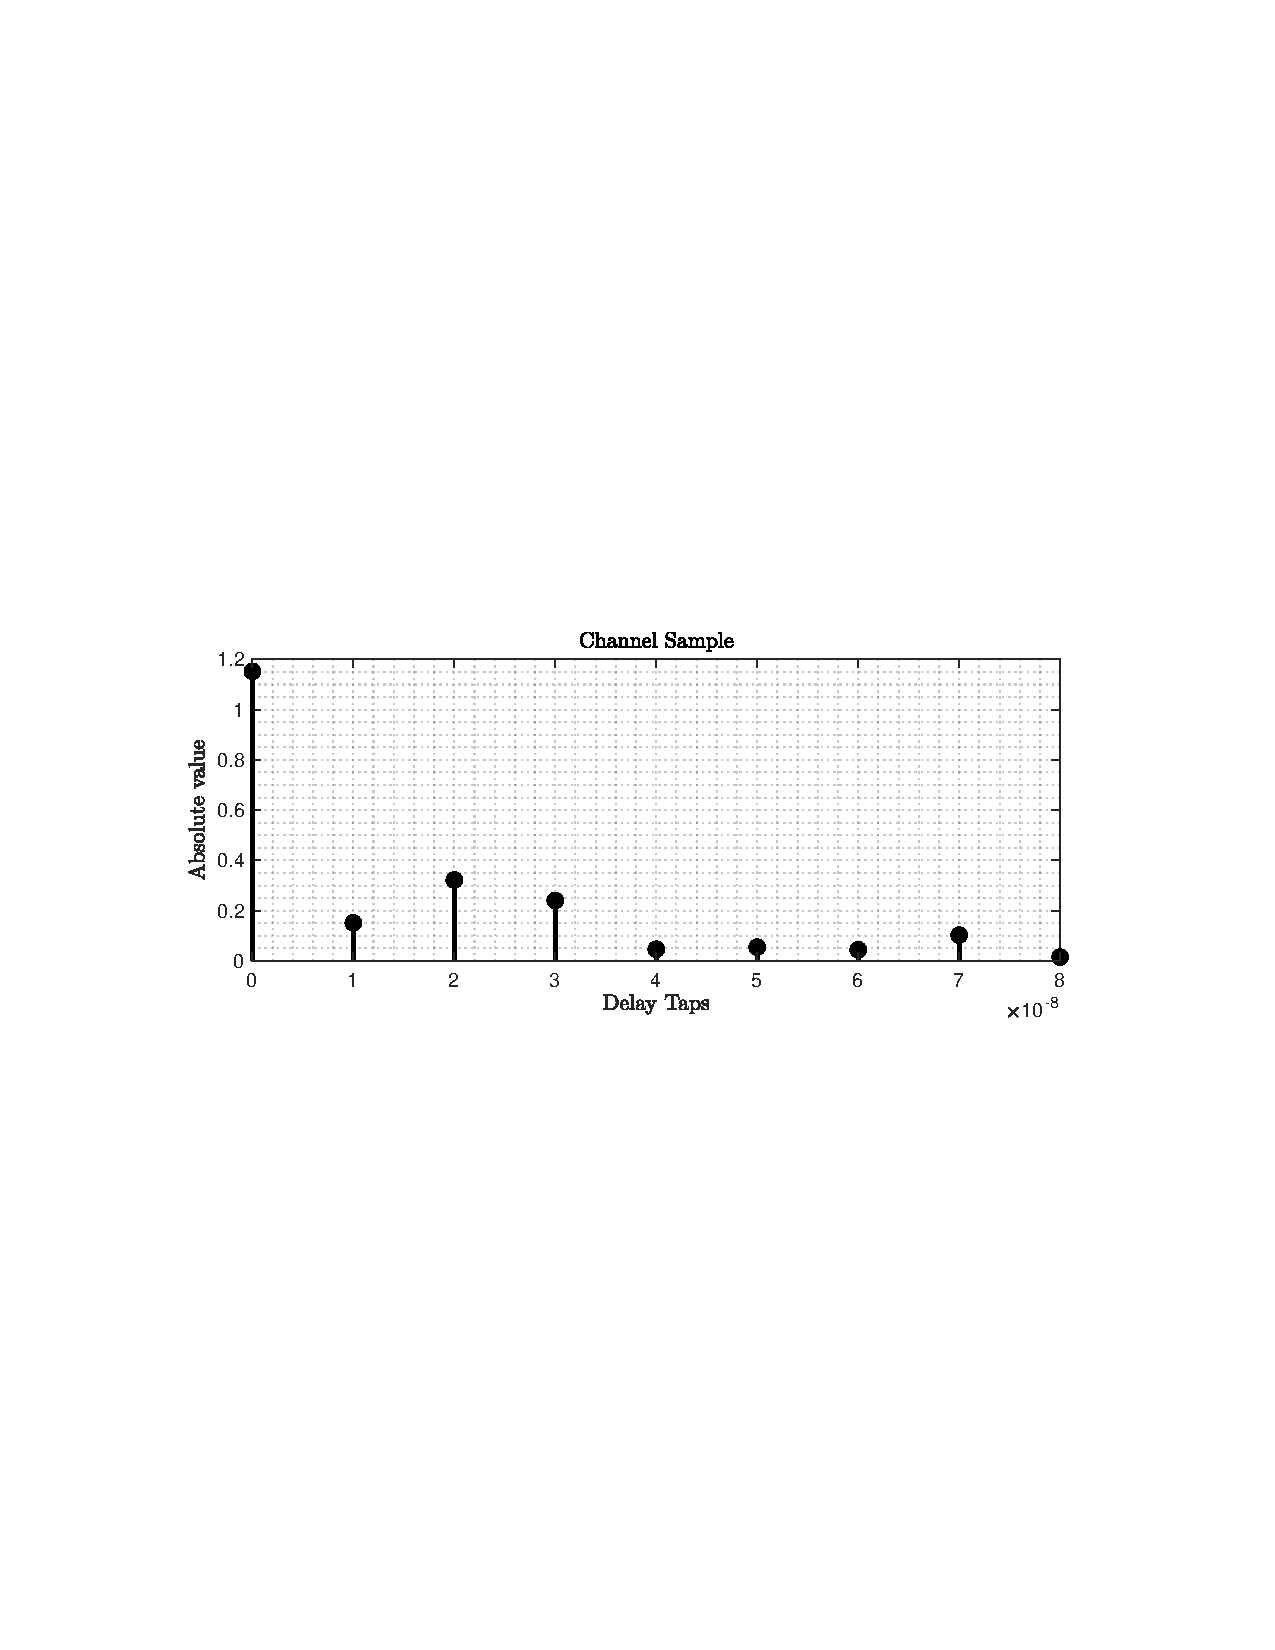
\includegraphics[height = 10cm]{figures/TimeSample.pdf}
%     \caption{Data Rate of User 1 versus its Distance from AP for Single Antenna Per User}
%     \label{fig:data-rate-distance-single}
% \end{figure}

% \begin{figure}
%     \centering
%     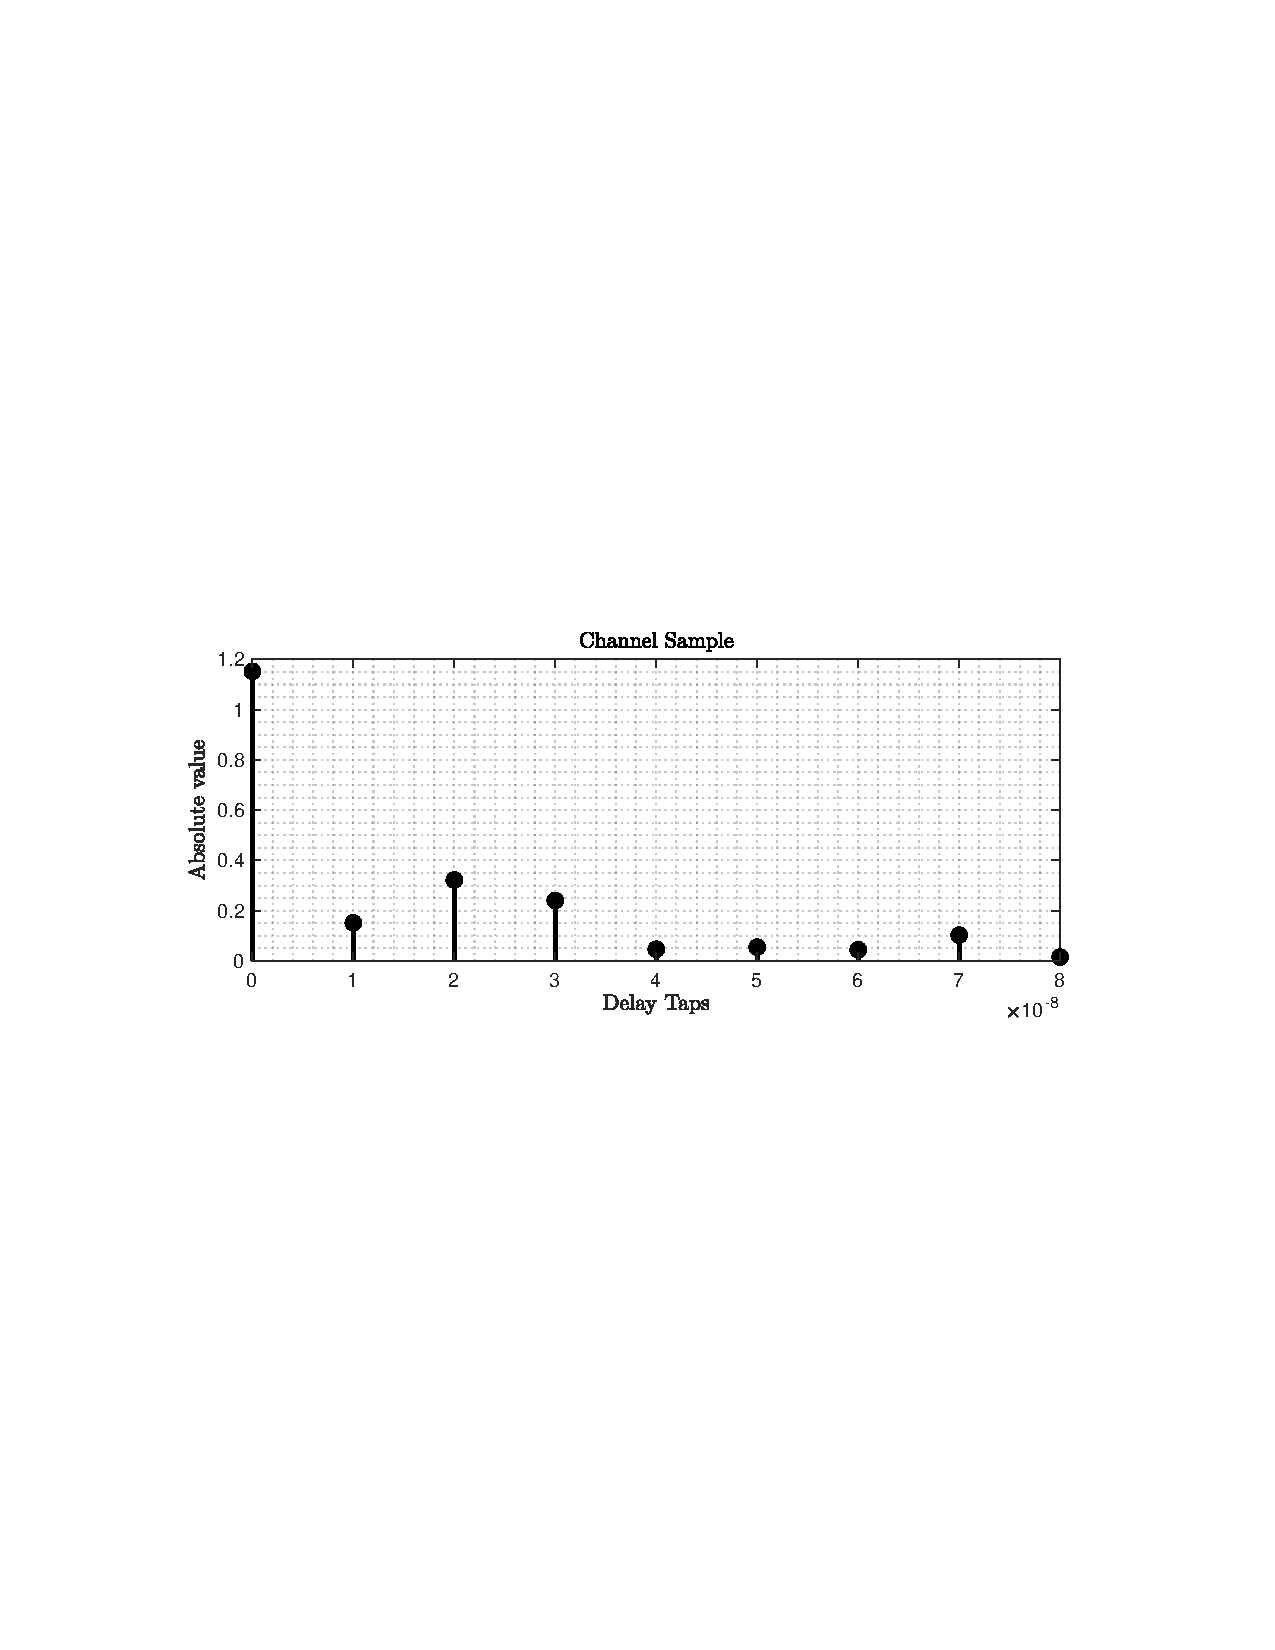
\includegraphics[height = 10cm]{figures/TimeSample.pdf}
%     \caption{Data Rate versus Number of AP antennas}
%     \label{fig:data-rate-AP-antennas-single}
% \end{figure}

% \begin{table}[t]
%     \caption{Experiment Scenarios for Multiple Antennas Per User}
%     \centering
%     \begin{tabular}{|c|c|}
%     \hline
%        & \\
%        & \\
%        & \\
%        & \\
%        &
%     \end{tabular}
%     \label{tab:scearios-multi}
% \end{table}

% \begin{figure}
%     \centering
%     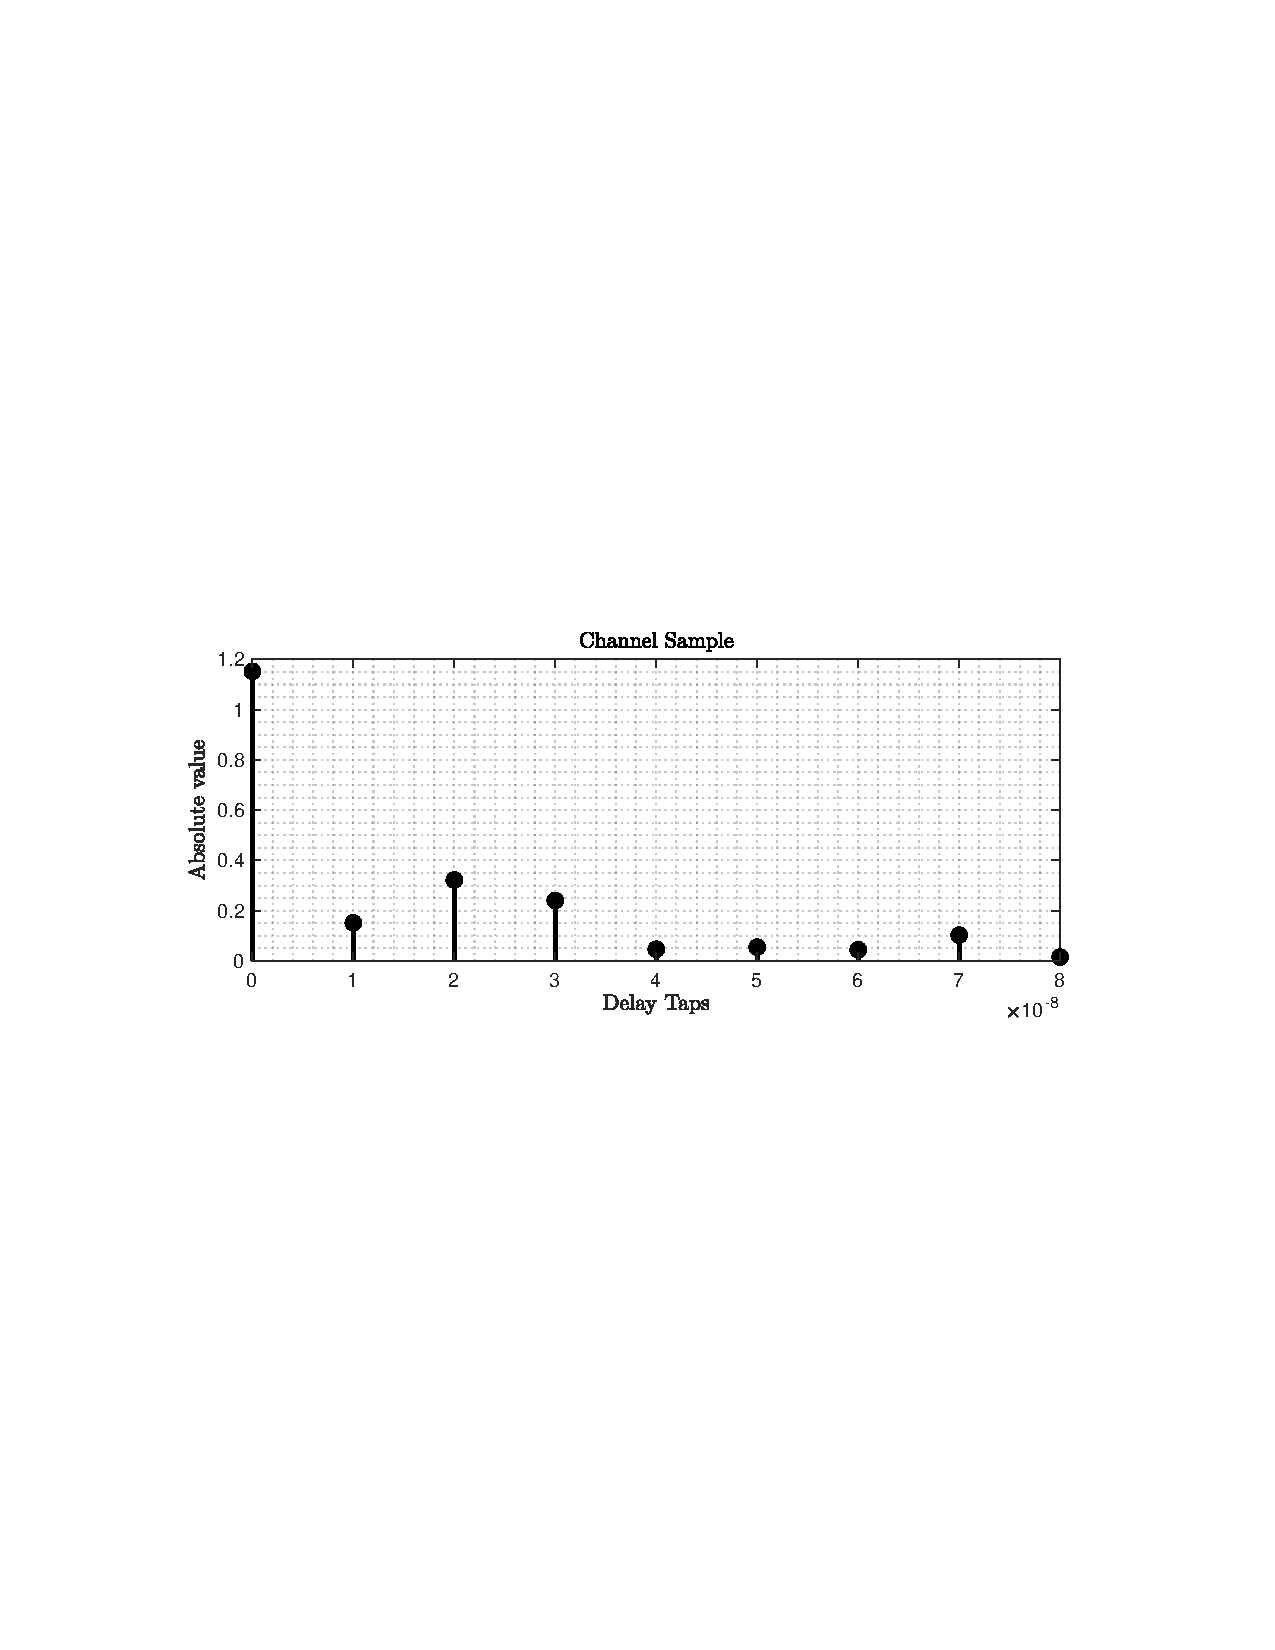
\includegraphics[height = 10cm]{figures/TimeSample.pdf}
%     \caption{Data Rate versus Number of User Antennas}
%     \label{fig:data-rate-user-antennas-multi}
% \end{figure}

% describe simulation environment: provide tables for parameters used 
In our experimental setup, we simulate a virtual reality (VR) gaming environment involving \( N \) users, each engaging in a distributed rendering task. These users, equipped with VR glasses, receive fragmented visual perspectives of a virtual room. We define \( L_{xu} \) as a 1x\( N \) array, representing the number of antennas at each user's device. Additionally, the access point (AP) is equipped with \( L_y \) antennas. The spatial positioning of users relative to the AP is modeled through a uniform random distribution, with distances ranging between \( d_{\text{min}} \) and \( d_{\text{max}} \). For the characterization of channel impulse responses between user devices and the AP, we utilize a dataset of over 10,000 channel realizations provided by Samsung. These realizations are based on WiFi 802.11ax standards \cite{802.11ax}, specifically tailored for model B (indoor residential) and model D (indoor office) scenarios. At any given moment, our experimental framework randomly selects one of these channel impulse responses for each pairing of the user device antenna and AP antenna. We multiply an additional components for path loss and shadow fading. We use the following combination of path loss and shadow fading loss:
\begin{equation}
    \begin{aligned}
        L(d) &= L_{path}(d) + L_{shadow}(d) \quad \textrm{dB}  \qquad \qquad d \leq d_{break} \\
    &= L_{path}(d_{break}) + L_{shadow}(d_{break}) + \\ & \qquad \qquad \qquad 35 \: \operatorname{log}_{10}(\frac{d}{d_{break}}) \quad \textrm{dB}  \qquad d>d_{break}
    \end{aligned}
\end{equation}
where the break-point distance is $d_{break} = 5\:m$, and 
\begin{align}
    L_{path} =  20 \: \operatorname{log}_{10}(f) + 20\: \operatorname{log}_{10}(d)  - 147.5 \textrm{dB}
\end{align}
and $L_{shadow}$ is a random log-normal variable sampled from $\frac{1}{\sqrt{2 \pi \sigma^{2}_{z}}}\exp{-(L_{shadow}(d)^{2}/(2\sigma^{2}_{z}))}$, $\sigma_{z}$ is $3 \textrm{dB}$ before breakpoint distance and $4 dB$ after the breakpoint. The channel delay taps are spaced 10 ns apart, hence the channel bandwidth is 100 MHz. In our experiments,we use the center frequency $f_{c}=5 GHz$ and vary the Fast Fourier Transform length $(fft_{length})$. Fig.~\ref{fig:channel-samples} shows an instance of the channel impulse responses used in the experiments. The parameters used for the experiments are tabulated in Table~\ref{tab:experiment-parameters}. We vary the transmit Signal-to-Noise Ratio (SNR) values and assess the resultant data rates achieved by both the baseline OFDM-based system and our proposed GDFE-based algorithm. Conversely, by setting variable minimum required data rates, we evaluate and compare the power consumption metrics for both the proposed algorithm and the baseline system. The ranges over which each of these parameters is varied are systematically tabulated for clarity and ease of reference.

% provide table and graph for results
Table \ref{tab:scearios-single} shows 2 instances of the experiment results using varying parameters. As we see from the first column, for the same data rates, the proposed algorithm consumes an order of magnitude less relative energy as compared to OFDM baselines. This shows that, even in the case where the total number of antennas at all users (2) is equal to the total number of antennas at the AP (2), harsh channel conditions and crosstalk between the subchannels lead to significant energy savings compared to OFDM, when using the proposed non-linear feedback-based algorithm. The second column stresses the channel further, i.e. forces it into a low-rank situation where the total number of antennas at the users (3) is less than the total number of antennas at the AP (2). Row lank regimes are where we see the massive benefit of using GDFE-based power allocation. This is aided by time sharing between users and thus simultaneous power allocation in the same time and frequency slot, which OFDM is incapable of. We achieve, on an average, 2 times the data rate at half the energy requirement.

Table~\ref{tab:energy-compare} demonstrates the proposed algorithm's superiority over the baseline OFDM in power efficiency across various AP antenna counts, maintaining a fixed data rate of 200 Mbps/user. The power savings become more pronounced as AP antennas decrease, attributed to the channel's lower rank in these scenarios, highlighting the algorithm's effectiveness in energy conservation under channel constrains. For the last row, where the number of antennas at AP (4) exceeds the number of user antennas (3), we see that the GDFE-based algorithm takes advantage of the crosstalk in the channel and achieves the required data rates at significantly lower energy compared to OFDM. 

Fig.~\ref{fig:data-rate-snr-single} shows the sum rate across 3 users located at equal distances of 3 m from the AP, as a function of SNR (dB). We see that the slope of increase of the data rates for the proposed algorithm is significantly higher than that for the OFDM-based current Wi-Fi algorithm. The inability of the OFDM-based system to utilize crosstalk between the channels is evident, and this crosstalk is utilized by the proposed algorithm to achieve high data rates, especially at high SNR values. There is time sharing between the three users. The first user has to suffer in data rates by treating the other two user's signals as noise, and the second user does this for the third user's signal. However, the third user gets to fully exploit all the available dimensions, which contributes to the high data rates. 

Fig.~\ref{fig:data-rate-fft-single} and Fig.~\ref{fig:data-rate-farthest-fft-single} compare the spectral efficiencies of a proposed algorithm against current Wi-Fi OFDM in equidistant users (3m, 3m, 3m) and non-equidistant users (3m, 5m, 8m) scenarios. As per Fig.~\ref{fig:data-rate-fft-single}, the proposed algorithm achieves 15 bits/s/Hz sum rates (500 Mbps/user) with FFT lengths ≥1024, outperforming OFDM's 11 bits/s/Hz. In Fig.~\ref{fig:data-rate-farthest-fft-single}, i.e., in non-equidistant setups, it ensures even the farthest user achieves equal data rates despite higher path losses, leveraging GDFE-based noise cancellation and time-sharing. The OFDM algorithm, which uses the water-filling algorithm for power allocation, fails to achieve this and hence the farthest user has the worst data rates of 2.3 bits/s/Hz at saturation. This demonstrates the proposed solution's superiority in energy and data rate efficiency, especially in low-rank channel conditions, making it a promising alternative to current Wi-Fi standards.

\section{Conclusion and Future Work}

% repeat proposed solution achievements from intro section
In this paper, we propose a novel Generalized Decision Feedback Equalizer (GDFE) strategy for power allocation that significantly enhances data rates and energy efficiency in low-rank channel conditions, which are particularly challenging for Extended Reality (XR) applications. Our comprehensive performance evaluation demonstrates that this approach markedly outperforms existing Wi-Fi methods, offering a promising solution for uplink communications in XR systems. Future directions include the integration of adaptive mechanisms and machine learning models to optimize power allocation dynamically, catering to real-time changes in channel conditions and further boosting the system's performance.

\footnotesize
\bibliographystyle{IEEEtran}
\bibliography{refs.bib}

\end{document}
